\documentclass[twoside]{article}

% Packages required by doxygen
\usepackage{calc}
\usepackage{doxygen}
\usepackage{graphicx}
\usepackage[utf8]{inputenc}
\usepackage{makeidx}
\usepackage{multicol}
\usepackage{multirow}
\usepackage{textcomp}
\usepackage[table]{xcolor}

% Font selection
\usepackage[T1]{fontenc}
\usepackage{mathptmx}
\usepackage[scaled=.90]{helvet}
\usepackage{courier}
\usepackage{amssymb}
\usepackage{sectsty}
\renewcommand{\familydefault}{\sfdefault}
\allsectionsfont{%
  \fontseries{bc}\selectfont%
  \color{darkgray}%
}
\renewcommand{\DoxyLabelFont}{%
  \fontseries{bc}\selectfont%
  \color{darkgray}%
}

% Page & text layout
\usepackage{geometry}
\geometry{%
  letterpaper,%
  top=2.5cm,%
  bottom=2.5cm,%
  left=2.5cm,%
  right=2.5cm%
}
\tolerance=750
\hfuzz=15pt
\hbadness=750
\setlength{\emergencystretch}{15pt}
\setlength{\parindent}{0cm}
\setlength{\parskip}{0.2cm}
\makeatletter
\renewcommand{\paragraph}{%
  \@startsection{paragraph}{4}{0ex}{-1.0ex}{1.0ex}{%
    \normalfont\normalsize\bfseries\SS@parafont%
  }%
}
\renewcommand{\subparagraph}{%
  \@startsection{subparagraph}{5}{0ex}{-1.0ex}{1.0ex}{%
    \normalfont\normalsize\bfseries\SS@subparafont%
  }%
}
\makeatother

% Headers & footers
\usepackage{fancyhdr}
\pagestyle{fancyplain}
\fancyhead[LE]{\fancyplain{}{\bfseries\thepage}}
\fancyhead[CE]{\fancyplain{}{}}
\fancyhead[RE]{\fancyplain{}{\bfseries\leftmark}}
\fancyhead[LO]{\fancyplain{}{\bfseries\rightmark}}
\fancyhead[CO]{\fancyplain{}{}}
\fancyhead[RO]{\fancyplain{}{\bfseries\thepage}}
\fancyfoot[LE]{\fancyplain{}{}}
\fancyfoot[CE]{\fancyplain{}{}}
\fancyfoot[RE]{\fancyplain{}{\bfseries\scriptsize Generated on Thu Dec 12 2013 13:15:24 for Ruminate by Doxygen }}
\fancyfoot[LO]{\fancyplain{}{\bfseries\scriptsize Generated on Thu Dec 12 2013 13:15:24 for Ruminate by Doxygen }}
\fancyfoot[CO]{\fancyplain{}{}}
\fancyfoot[RO]{\fancyplain{}{}}
\renewcommand{\footrulewidth}{0.4pt}
\renewcommand{\sectionmark}[1]{%
  \markright{\thesection\ #1}%
}

% Indices & bibliography
\usepackage{natbib}
\usepackage[titles]{tocloft}
\setcounter{tocdepth}{3}
\setcounter{secnumdepth}{5}
\makeindex

% Hyperlinks (required, but should be loaded last)
\usepackage{ifpdf}
\ifpdf
  \usepackage[pdftex,pagebackref=true]{hyperref}
\else
  \usepackage[ps2pdf,pagebackref=true]{hyperref}
\fi
\hypersetup{%
  colorlinks=true,%
  linkcolor=blue,%
  citecolor=blue,%
  unicode%
}

% Custom commands
\newcommand{\clearemptydoublepage}{%
  \newpage{\pagestyle{empty}\cleardoublepage}%
}


%===== C O N T E N T S =====

\begin{document}

% Titlepage & ToC
\hypersetup{pageanchor=false}
\pagenumbering{roman}
\begin{titlepage}
\vspace*{7cm}
\begin{center}%
{\Large Ruminate }\\
\vspace*{1cm}
{\large Generated by Doxygen 1.8.4}\\
\vspace*{0.5cm}
{\small Thu Dec 12 2013 13:15:24}\\
\end{center}
\end{titlepage}
\tableofcontents
\pagenumbering{arabic}
\hypersetup{pageanchor=true}

%--- Begin generated contents ---
\section{Main Page}
\label{index}\hypertarget{index}{}Ruminate is an \href{http://en.wikipedia.org/wiki/Introspection_(computer_science)}{\tt introspective} library for C.

It is a relatively new project and very much a work in progress.

More documentation to come later.

See \hyperlink{ruminate_2ruminate_8h_a1d17861ce087a20632d29f3b6e09dccb}{ruminate\-\_\-get\-\_\-type()} 
\section{Todo List}
\label{todo}
\hypertarget{todo}{}

\begin{DoxyRefList}
\item[\label{todo__todo000007}%
\hypertarget{todo__todo000007}{}%
Member \hyperlink{type_8h_a98af7901cdefcac1a911764c15d636f0}{r\-\_\-type\-\_\-size} (\hyperlink{struct_r_type}{R\-Type} $\ast$, G\-Error $\ast$$\ast$error)]Document this  
\item[\label{todo__todo000001}%
\hypertarget{todo__todo000001}{}%
Member \hyperlink{struct_r_aggregate_member_a48fc0de0e9dc5bfba78304194536c919}{R\-Aggregate\-Member\-:\-:r\-\_\-aggregate\-\_\-member\-\_\-name} (\hyperlink{struct_r_aggregate_member}{R\-Aggregate\-Member} $\ast$member, G\-Error $\ast$$\ast$error)]Function argument names return {\ttfamily \char`\"{}\char`\"{}}. I'm not sure it's even possible to get these, so this feature might go away.  
\item[\label{todo__todo000008}%
\hypertarget{todo__todo000008}{}%
Member \hyperlink{struct_r_typedef_type_afa3538fc4df5050ba3df60547f36536c}{R\-Typedef\-Type\-:\-:r\-\_\-typedef\-\_\-type\-\_\-canonical} (\hyperlink{struct_r_typedef_type}{R\-Typedef\-Type} $\ast$, G\-Error $\ast$$\ast$error)]Be able to single step through non-\/canonical types of an \hyperlink{struct_r_typedef_type}{R\-Typedef\-Type}.  
\item[\label{todo__todo000002}%
\hypertarget{todo__todo000002}{}%
Member \hyperlink{ruminate_2ruminate_8h_ace611a174dd203875ab2ea450ed0080b}{ruminate\-\_\-backtrace} (G\-Error $\ast$$\ast$error)]This method should return a G\-Ptr\-Array rather than a custom list implementation.  
\item[\label{todo__todo000003}%
\hypertarget{todo__todo000003}{}%
Member \hyperlink{ruminate_2ruminate_8h_aeb372297a5feab4cb66e051256fd3a22}{ruminate\-\_\-get\-\_\-type\-\_\-by\-\_\-variable\-\_\-name} (const char $\ast$, G\-Error $\ast$$\ast$)]document 
\end{DoxyRefList}
\section{Hierarchical Index}
\subsection{Class Hierarchy}
This inheritance list is sorted roughly, but not completely, alphabetically\-:\begin{DoxyCompactList}
\item \contentsline{section}{R\-Frame}{\pageref{struct_r_frame}}{}
\item \contentsline{section}{R\-Frame\-List}{\pageref{struct_r_frame_list}}{}
\item \contentsline{section}{R\-String}{\pageref{struct_r_string}}{}
\item \contentsline{section}{R\-Type}{\pageref{struct_r_type}}{}
\begin{DoxyCompactList}
\item \contentsline{section}{R\-Aggregate\-Type}{\pageref{struct_r_aggregate_type}}{}
\begin{DoxyCompactList}
\item \contentsline{section}{R\-Function\-Type}{\pageref{struct_r_function_type}}{}
\end{DoxyCompactList}
\item \contentsline{section}{R\-Array\-Type}{\pageref{struct_r_array_type}}{}
\item \contentsline{section}{R\-Builtin\-Type}{\pageref{struct_r_builtin_type}}{}
\item \contentsline{section}{R\-Pointer\-Type}{\pageref{struct_r_pointer_type}}{}
\item \contentsline{section}{R\-Typedef\-Type}{\pageref{struct_r_typedef_type}}{}
\end{DoxyCompactList}
\item \contentsline{section}{R\-Type\-Member}{\pageref{struct_r_type_member}}{}
\begin{DoxyCompactList}
\item \contentsline{section}{R\-Aggregate\-Member}{\pageref{struct_r_aggregate_member}}{}
\begin{DoxyCompactList}
\item \contentsline{section}{R\-Enum\-Member}{\pageref{struct_r_enum_member}}{}
\end{DoxyCompactList}
\end{DoxyCompactList}
\end{DoxyCompactList}

\section{Class Index}
\subsection{Class List}
Here are the classes, structs, unions and interfaces with brief descriptions\-:\begin{DoxyCompactList}
\item\contentsline{section}{\hyperlink{struct_r_aggregate_member}{R\-Aggregate\-Member} \\*An opaque struct representing a aggregate member }{\pageref{struct_r_aggregate_member}}{}
\item\contentsline{section}{\hyperlink{struct_r_aggregate_type}{R\-Aggregate\-Type} \\*An opaque struct representing a aggregate type }{\pageref{struct_r_aggregate_type}}{}
\item\contentsline{section}{\hyperlink{struct_r_array_type}{R\-Array\-Type} \\*An opaque struct representing an array type }{\pageref{struct_r_array_type}}{}
\item\contentsline{section}{\hyperlink{struct_r_builtin_type}{R\-Builtin\-Type} \\*An opaque struct representing a builtin type }{\pageref{struct_r_builtin_type}}{}
\item\contentsline{section}{\hyperlink{struct_r_enum_member}{R\-Enum\-Member} \\*An opaque struct representing an enum member }{\pageref{struct_r_enum_member}}{}
\item\contentsline{section}{\hyperlink{struct_r_frame}{R\-Frame} \\*An opaque struct representing a call stack frame }{\pageref{struct_r_frame}}{}
\item\contentsline{section}{\hyperlink{struct_r_frame_list}{R\-Frame\-List} \\*An opaque struct representing a call stack }{\pageref{struct_r_frame_list}}{}
\item\contentsline{section}{\hyperlink{struct_r_function_type}{R\-Function\-Type} \\*An opaque struct representing a function }{\pageref{struct_r_function_type}}{}
\item\contentsline{section}{\hyperlink{struct_r_pointer_type}{R\-Pointer\-Type} \\*An opaque struct representing a pointer to another type }{\pageref{struct_r_pointer_type}}{}
\item\contentsline{section}{\hyperlink{struct_r_string}{R\-String} \\*An opaque struct representing a string }{\pageref{struct_r_string}}{}
\item\contentsline{section}{\hyperlink{struct_r_type}{R\-Type} \\*An opaque struct representing a type }{\pageref{struct_r_type}}{}
\item\contentsline{section}{\hyperlink{struct_r_typedef_type}{R\-Typedef\-Type} \\*An opaque struct representing a typedef'ed type }{\pageref{struct_r_typedef_type}}{}
\item\contentsline{section}{\hyperlink{struct_r_type_member}{R\-Type\-Member} \\*An opaque struct representing a type member }{\pageref{struct_r_type_member}}{}
\end{DoxyCompactList}

\section{File Index}
\subsection{File List}
Here is a list of all documented files with brief descriptions\-:\begin{DoxyCompactList}
\item\contentsline{section}{\hyperlink{ruminate_8h}{ruminate.\-h} \\*The only file you should need to include }{\pageref{ruminate_8h}}{}
\item\contentsline{section}{ruminate/\hyperlink{aggregate__member_8h}{aggregate\-\_\-member.\-h} \\*Aggregate members }{\pageref{aggregate__member_8h}}{}
\item\contentsline{section}{ruminate/\hyperlink{aggregate__type_8h}{aggregate\-\_\-type.\-h} \\*Aggregate types }{\pageref{aggregate__type_8h}}{}
\item\contentsline{section}{ruminate/\hyperlink{builtin__type_8h}{builtin\-\_\-type.\-h} \\*Built-\/in types }{\pageref{builtin__type_8h}}{}
\item\contentsline{section}{ruminate/\hyperlink{errors_8h}{errors.\-h} \\*Error handling facilities }{\pageref{errors_8h}}{}
\item\contentsline{section}{ruminate/\hyperlink{memory_8h}{memory.\-h} \\*Typed reference counted memory allocator }{\pageref{memory_8h}}{}
\item\contentsline{section}{ruminate/\hyperlink{ruminate_2ruminate_8h}{ruminate.\-h} \\*Top-\/level and utility functions }{\pageref{ruminate_2ruminate_8h}}{}
\item\contentsline{section}{ruminate/\hyperlink{type_8h}{type.\-h} \\*The top level of the ruminate type hierarchy }{\pageref{type_8h}}{}
\item\contentsline{section}{ruminate/\hyperlink{type__member_8h}{type\-\_\-member.\-h} \\*Type members }{\pageref{type__member_8h}}{}
\end{DoxyCompactList}

\section{Class Documentation}
\hypertarget{struct_r_aggregate_member}{\subsection{R\-Aggregate\-Member Struct Reference}
\label{struct_r_aggregate_member}\index{R\-Aggregate\-Member@{R\-Aggregate\-Member}}
}


An opaque struct representing a aggregate member.  




Inheritance diagram for R\-Aggregate\-Member\-:\nopagebreak
\begin{figure}[H]
\begin{center}
\leavevmode
\includegraphics[width=184pt]{struct_r_aggregate_member__inherit__graph}
\end{center}
\end{figure}
\subsubsection*{Public Member Functions}
\begin{DoxyCompactItemize}
\item 
\hyperlink{aggregate__member_8h_ae66a822b4bce9e1559fef33422de505c}{R\-Aggregate\-Member\-Id} \hyperlink{struct_r_aggregate_member_a3d8b736967820633c1fcd3c91958cdea}{r\-\_\-aggregate\-\_\-member\-\_\-id} (\hyperlink{struct_r_aggregate_member}{R\-Aggregate\-Member} $\ast$member, G\-Error $\ast$$\ast$error)
\begin{DoxyCompactList}\small\item\em Get the real type identifier of this aggregate member. \end{DoxyCompactList}\item 
\hyperlink{struct_r_string}{R\-String} $\ast$ \hyperlink{struct_r_aggregate_member_a48fc0de0e9dc5bfba78304194536c919}{r\-\_\-aggregate\-\_\-member\-\_\-name} (\hyperlink{struct_r_aggregate_member}{R\-Aggregate\-Member} $\ast$member, G\-Error $\ast$$\ast$error)
\begin{DoxyCompactList}\small\item\em Get the name of this aggregate member. \end{DoxyCompactList}\end{DoxyCompactItemize}


\subsubsection{Detailed Description}
An opaque struct representing a aggregate member. 

\begin{DoxySeeAlso}{See Also}
\hyperlink{struct_r_aggregate_type}{R\-Aggregate\-Type} 
\end{DoxySeeAlso}


\subsubsection{Member Function Documentation}
\hypertarget{struct_r_aggregate_member_a3d8b736967820633c1fcd3c91958cdea}{\index{R\-Aggregate\-Member@{R\-Aggregate\-Member}!r\-\_\-aggregate\-\_\-member\-\_\-id@{r\-\_\-aggregate\-\_\-member\-\_\-id}}
\index{r\-\_\-aggregate\-\_\-member\-\_\-id@{r\-\_\-aggregate\-\_\-member\-\_\-id}!RAggregateMember@{R\-Aggregate\-Member}}
\paragraph[{r\-\_\-aggregate\-\_\-member\-\_\-id}]{\setlength{\rightskip}{0pt plus 5cm}{\bf R\-Aggregate\-Member\-Id} r\-\_\-aggregate\-\_\-member\-\_\-id (
\begin{DoxyParamCaption}
\item[{{\bf R\-Aggregate\-Member} $\ast$}]{member, }
\item[{G\-Error $\ast$$\ast$}]{error}
\end{DoxyParamCaption}
)}}\label{struct_r_aggregate_member_a3d8b736967820633c1fcd3c91958cdea}


Get the real type identifier of this aggregate member. 

\begin{DoxyReturn}{Returns}
the real type of this aggregate member 
\end{DoxyReturn}

\begin{DoxyParams}[1]{Parameters}
\mbox{\tt in}  & {\em member} & the aggregate member to get the id of \\
\hline
\mbox{\tt out}  & {\em error} & see \hyperlink{errors_8h}{errors.\-h} \\
\hline
\end{DoxyParams}
\hypertarget{struct_r_aggregate_member_a48fc0de0e9dc5bfba78304194536c919}{\index{R\-Aggregate\-Member@{R\-Aggregate\-Member}!r\-\_\-aggregate\-\_\-member\-\_\-name@{r\-\_\-aggregate\-\_\-member\-\_\-name}}
\index{r\-\_\-aggregate\-\_\-member\-\_\-name@{r\-\_\-aggregate\-\_\-member\-\_\-name}!RAggregateMember@{R\-Aggregate\-Member}}
\paragraph[{r\-\_\-aggregate\-\_\-member\-\_\-name}]{\setlength{\rightskip}{0pt plus 5cm}{\bf R\-String} $\ast$ r\-\_\-aggregate\-\_\-member\-\_\-name (
\begin{DoxyParamCaption}
\item[{{\bf R\-Aggregate\-Member} $\ast$}]{member, }
\item[{G\-Error $\ast$$\ast$}]{error}
\end{DoxyParamCaption}
)}}\label{struct_r_aggregate_member_a48fc0de0e9dc5bfba78304194536c919}


Get the name of this aggregate member. 

\begin{DoxyReturn}{Returns}
a \hyperlink{struct_r_string}{R\-String} containing the name of this aggregate member 
\end{DoxyReturn}
\begin{DoxyRefDesc}{Todo}
\item[\hyperlink{todo__todo000001}{Todo}]Function argument names return {\ttfamily \char`\"{}\char`\"{}}. I'm not sure it's even possible to get these, so this feature might go away. \end{DoxyRefDesc}

\begin{DoxyParams}[1]{Parameters}
\mbox{\tt in}  & {\em member} & the aggregate member to get the name of \\
\hline
\mbox{\tt in}  & {\em error} & see \hyperlink{errors_8h}{errors.\-h} \\
\hline
\end{DoxyParams}


The documentation for this struct was generated from the following file\-:\begin{DoxyCompactItemize}
\item 
ruminate/\hyperlink{aggregate__member_8h}{aggregate\-\_\-member.\-h}\end{DoxyCompactItemize}

\hypertarget{struct_r_aggregate_type}{\subsection{R\-Aggregate\-Type Struct Reference}
\label{struct_r_aggregate_type}\index{R\-Aggregate\-Type@{R\-Aggregate\-Type}}
}


An opaque struct representing a aggregate type.  




Inheritance diagram for R\-Aggregate\-Type\-:\nopagebreak
\begin{figure}[H]
\begin{center}
\leavevmode
\includegraphics[width=170pt]{struct_r_aggregate_type__inherit__graph}
\end{center}
\end{figure}
\subsubsection*{Public Member Functions}
\begin{DoxyCompactItemize}
\item 
\hyperlink{aggregate__type_8h_ae208e3e28b5dcedb640f7f4b0581d61a}{R\-Aggregate\-Type\-Id} \hyperlink{struct_r_aggregate_type_a3ad647b94dd87268b91e92f630b84726}{r\-\_\-aggregate\-\_\-type\-\_\-id} (\hyperlink{struct_r_aggregate_type}{R\-Aggregate\-Type} $\ast$type, G\-Error $\ast$$\ast$error)
\begin{DoxyCompactList}\small\item\em Get the aggregate type identifier of this aggregate type. \end{DoxyCompactList}\item 
size\-\_\-t \hyperlink{struct_r_aggregate_type_a193960ea5996d7c1c7935b1525cf64c9}{r\-\_\-aggregate\-\_\-type\-\_\-nmembers} (\hyperlink{struct_r_aggregate_type}{R\-Aggregate\-Type} $\ast$type, G\-Error $\ast$$\ast$error)
\begin{DoxyCompactList}\small\item\em Get the number of members in this aggregate type. \end{DoxyCompactList}\item 
\hyperlink{struct_r_aggregate_member}{R\-Aggregate\-Member} $\ast$ \hyperlink{struct_r_aggregate_type_aea94153a211184cee889e445a7dd003a}{r\-\_\-aggregate\-\_\-type\-\_\-member\-\_\-at} (\hyperlink{struct_r_aggregate_type}{R\-Aggregate\-Type} $\ast$type, size\-\_\-t index, G\-Error $\ast$$\ast$error)
\begin{DoxyCompactList}\small\item\em Get a aggregate's member at a specified index. \end{DoxyCompactList}\end{DoxyCompactItemize}


\subsubsection{Detailed Description}
An opaque struct representing a aggregate type. 

This aggregate type can be safely cast to it's sub-\/type which can be determined by using \hyperlink{struct_r_aggregate_type_a3ad647b94dd87268b91e92f630b84726}{r\-\_\-aggregate\-\_\-type\-\_\-id()} 

\subsubsection{Member Function Documentation}
\hypertarget{struct_r_aggregate_type_a3ad647b94dd87268b91e92f630b84726}{\index{R\-Aggregate\-Type@{R\-Aggregate\-Type}!r\-\_\-aggregate\-\_\-type\-\_\-id@{r\-\_\-aggregate\-\_\-type\-\_\-id}}
\index{r\-\_\-aggregate\-\_\-type\-\_\-id@{r\-\_\-aggregate\-\_\-type\-\_\-id}!RAggregateType@{R\-Aggregate\-Type}}
\paragraph[{r\-\_\-aggregate\-\_\-type\-\_\-id}]{\setlength{\rightskip}{0pt plus 5cm}{\bf R\-Aggregate\-Type\-Id} r\-\_\-aggregate\-\_\-type\-\_\-id (
\begin{DoxyParamCaption}
\item[{{\bf R\-Aggregate\-Type} $\ast$}]{type, }
\item[{G\-Error $\ast$$\ast$}]{error}
\end{DoxyParamCaption}
)}}\label{struct_r_aggregate_type_a3ad647b94dd87268b91e92f630b84726}


Get the aggregate type identifier of this aggregate type. 

The R\-Aggregate\-Type\-Id of this \hyperlink{struct_r_aggregate_type}{R\-Aggregate\-Type} represents the child type of this \hyperlink{struct_r_aggregate_type}{R\-Aggregate\-Type}, and can be safely cast into that child type.

\begin{DoxyReturn}{Returns}
the child type of this aggregate type. 
\end{DoxyReturn}

\begin{DoxyParams}[1]{Parameters}
\mbox{\tt in}  & {\em type} & the aggregate type to retrieve the id of \\
\hline
\mbox{\tt out}  & {\em error} & see \hyperlink{errors_8h}{errors.\-h} \\
\hline
\end{DoxyParams}
\hypertarget{struct_r_aggregate_type_aea94153a211184cee889e445a7dd003a}{\index{R\-Aggregate\-Type@{R\-Aggregate\-Type}!r\-\_\-aggregate\-\_\-type\-\_\-member\-\_\-at@{r\-\_\-aggregate\-\_\-type\-\_\-member\-\_\-at}}
\index{r\-\_\-aggregate\-\_\-type\-\_\-member\-\_\-at@{r\-\_\-aggregate\-\_\-type\-\_\-member\-\_\-at}!RAggregateType@{R\-Aggregate\-Type}}
\paragraph[{r\-\_\-aggregate\-\_\-type\-\_\-member\-\_\-at}]{\setlength{\rightskip}{0pt plus 5cm}{\bf R\-Aggregate\-Member} $\ast$ r\-\_\-aggregate\-\_\-type\-\_\-member\-\_\-at (
\begin{DoxyParamCaption}
\item[{{\bf R\-Aggregate\-Type} $\ast$}]{type, }
\item[{size\-\_\-t}]{index, }
\item[{G\-Error $\ast$$\ast$}]{error}
\end{DoxyParamCaption}
)}}\label{struct_r_aggregate_type_aea94153a211184cee889e445a7dd003a}


Get a aggregate's member at a specified index. 

\begin{DoxyReturn}{Returns}
a \hyperlink{struct_r_aggregate_member}{R\-Aggregate\-Member} representing the member of this aggregate at index {\itshape index}. 
\end{DoxyReturn}

\begin{DoxyParams}[1]{Parameters}
\mbox{\tt in}  & {\em type} & the aggregate type to retrieve a member of \\
\hline
\mbox{\tt in}  & {\em index} & the index of the member \\
\hline
\mbox{\tt out}  & {\em error} & see \hyperlink{errors_8h}{errors.\-h} \\
\hline
\end{DoxyParams}
\hypertarget{struct_r_aggregate_type_a193960ea5996d7c1c7935b1525cf64c9}{\index{R\-Aggregate\-Type@{R\-Aggregate\-Type}!r\-\_\-aggregate\-\_\-type\-\_\-nmembers@{r\-\_\-aggregate\-\_\-type\-\_\-nmembers}}
\index{r\-\_\-aggregate\-\_\-type\-\_\-nmembers@{r\-\_\-aggregate\-\_\-type\-\_\-nmembers}!RAggregateType@{R\-Aggregate\-Type}}
\paragraph[{r\-\_\-aggregate\-\_\-type\-\_\-nmembers}]{\setlength{\rightskip}{0pt plus 5cm}size\-\_\-t r\-\_\-aggregate\-\_\-type\-\_\-nmembers (
\begin{DoxyParamCaption}
\item[{{\bf R\-Aggregate\-Type} $\ast$}]{type, }
\item[{G\-Error $\ast$$\ast$}]{error}
\end{DoxyParamCaption}
)}}\label{struct_r_aggregate_type_a193960ea5996d7c1c7935b1525cf64c9}


Get the number of members in this aggregate type. 

\begin{DoxyReturn}{Returns}
the number of members in this aggregate type. 
\end{DoxyReturn}

\begin{DoxyParams}[1]{Parameters}
\mbox{\tt in}  & {\em type} & the type to get the number of members of \\
\hline
\mbox{\tt out}  & {\em error} & see \hyperlink{errors_8h}{errors.\-h} \\
\hline
\end{DoxyParams}


The documentation for this struct was generated from the following file\-:\begin{DoxyCompactItemize}
\item 
ruminate/\hyperlink{aggregate__type_8h}{aggregate\-\_\-type.\-h}\end{DoxyCompactItemize}

\hypertarget{struct_r_array_type}{\subsection{R\-Array\-Type Struct Reference}
\label{struct_r_array_type}\index{R\-Array\-Type@{R\-Array\-Type}}
}


An opaque struct representing an array type.  




Inheritance diagram for R\-Array\-Type\-:\nopagebreak
\begin{figure}[H]
\begin{center}
\leavevmode
\includegraphics[width=148pt]{struct_r_array_type__inherit__graph}
\end{center}
\end{figure}
\subsubsection*{Public Member Functions}
\begin{DoxyCompactItemize}
\item 
size\-\_\-t \hyperlink{struct_r_array_type_a91fdc9370c7373eae37b12372042a9d6}{r\-\_\-array\-\_\-type\-\_\-size} (\hyperlink{struct_r_array_type}{R\-Array\-Type} $\ast$type, G\-Error $\ast$$\ast$error)
\begin{DoxyCompactList}\small\item\em Get the size of this array. \end{DoxyCompactList}\item 
\hyperlink{struct_r_type_member}{R\-Type\-Member} $\ast$ \hyperlink{struct_r_array_type_a7efce78c90306eca927204d10b72f4e4}{r\-\_\-array\-\_\-type\-\_\-member\-\_\-at} (\hyperlink{struct_r_array_type}{R\-Array\-Type} $\ast$type, size\-\_\-t index, G\-Error $\ast$$\ast$error)
\begin{DoxyCompactList}\small\item\em Get the type of a member of this array. \end{DoxyCompactList}\end{DoxyCompactItemize}


\subsubsection{Detailed Description}
An opaque struct representing an array type. 

\subsubsection{Member Function Documentation}
\hypertarget{struct_r_array_type_a7efce78c90306eca927204d10b72f4e4}{\index{R\-Array\-Type@{R\-Array\-Type}!r\-\_\-array\-\_\-type\-\_\-member\-\_\-at@{r\-\_\-array\-\_\-type\-\_\-member\-\_\-at}}
\index{r\-\_\-array\-\_\-type\-\_\-member\-\_\-at@{r\-\_\-array\-\_\-type\-\_\-member\-\_\-at}!RArrayType@{R\-Array\-Type}}
\paragraph[{r\-\_\-array\-\_\-type\-\_\-member\-\_\-at}]{\setlength{\rightskip}{0pt plus 5cm}{\bf R\-Type\-Member} $\ast$ r\-\_\-array\-\_\-type\-\_\-member\-\_\-at (
\begin{DoxyParamCaption}
\item[{{\bf R\-Array\-Type} $\ast$}]{type, }
\item[{size\-\_\-t}]{index, }
\item[{G\-Error $\ast$$\ast$}]{error}
\end{DoxyParamCaption}
)}}\label{struct_r_array_type_a7efce78c90306eca927204d10b72f4e4}


Get the type of a member of this array. 

\begin{DoxyReturn}{Returns}
A \hyperlink{struct_r_type_member}{R\-Type\-Member} representing the type of the argument at index {\itshape index} 
\end{DoxyReturn}

\begin{DoxyParams}[1]{Parameters}
\mbox{\tt in}  & {\em type} & the type to get the member type of \\
\hline
\mbox{\tt in}  & {\em index} & the index in the array to get the member type of \\
\hline
\mbox{\tt out}  & {\em error} & see \hyperlink{errors_8h}{errors.\-h} \\
\hline
\end{DoxyParams}
\hypertarget{struct_r_array_type_a91fdc9370c7373eae37b12372042a9d6}{\index{R\-Array\-Type@{R\-Array\-Type}!r\-\_\-array\-\_\-type\-\_\-size@{r\-\_\-array\-\_\-type\-\_\-size}}
\index{r\-\_\-array\-\_\-type\-\_\-size@{r\-\_\-array\-\_\-type\-\_\-size}!RArrayType@{R\-Array\-Type}}
\paragraph[{r\-\_\-array\-\_\-type\-\_\-size}]{\setlength{\rightskip}{0pt plus 5cm}size\-\_\-t r\-\_\-array\-\_\-type\-\_\-size (
\begin{DoxyParamCaption}
\item[{{\bf R\-Array\-Type} $\ast$}]{type, }
\item[{G\-Error $\ast$$\ast$}]{error}
\end{DoxyParamCaption}
)}}\label{struct_r_array_type_a91fdc9370c7373eae37b12372042a9d6}


Get the size of this array. 

\begin{DoxyReturn}{Returns}
the size of the array 
\end{DoxyReturn}

\begin{DoxyParams}[1]{Parameters}
\mbox{\tt in}  & {\em type} & the type to get the size of \\
\hline
\mbox{\tt out}  & {\em error} & see \hyperlink{errors_8h}{errors.\-h} \\
\hline
\end{DoxyParams}


The documentation for this struct was generated from the following file\-:\begin{DoxyCompactItemize}
\item 
ruminate/array\-\_\-type.\-h\end{DoxyCompactItemize}

\hypertarget{struct_r_builtin_type}{\subsection{R\-Builtin\-Type Struct Reference}
\label{struct_r_builtin_type}\index{R\-Builtin\-Type@{R\-Builtin\-Type}}
}


An opaque struct representing a builtin type.  




Inheritance diagram for R\-Builtin\-Type\-:\nopagebreak
\begin{figure}[H]
\begin{center}
\leavevmode
\includegraphics[width=152pt]{struct_r_builtin_type__inherit__graph}
\end{center}
\end{figure}
\subsubsection*{Public Member Functions}
\begin{DoxyCompactItemize}
\item 
\hyperlink{builtin__type_8h_a245d1724f16dd995c090e6666722c80c}{R\-Builtin\-Type\-Id} \hyperlink{struct_r_builtin_type_afaf0b8970072c1587ebc7936eaccbcee}{r\-\_\-builtin\-\_\-type\-\_\-id} (\hyperlink{struct_r_builtin_type}{R\-Builtin\-Type} $\ast$type, G\-Error $\ast$$\ast$error)
\begin{DoxyCompactList}\small\item\em Get the builtin type identifier of this builtin type. \end{DoxyCompactList}\item 
bool \hyperlink{struct_r_builtin_type_a93b47b692eee1bdead79045599b47c1f}{r\-\_\-builtin\-\_\-type\-\_\-is\-\_\-signed} (\hyperlink{struct_r_builtin_type}{R\-Builtin\-Type} $\ast$type, G\-Error $\ast$$\ast$error)
\begin{DoxyCompactList}\small\item\em Determine if this type is signed. \end{DoxyCompactList}\item 
bool \hyperlink{struct_r_builtin_type_a539615767bc3af7470da1e73456bfe10}{r\-\_\-builtin\-\_\-type\-\_\-is\-\_\-unsigned} (\hyperlink{struct_r_builtin_type}{R\-Builtin\-Type} $\ast$type, G\-Error $\ast$$\ast$error)
\begin{DoxyCompactList}\small\item\em Determine if this type is unsigned. \end{DoxyCompactList}\end{DoxyCompactItemize}


\subsubsection{Detailed Description}
An opaque struct representing a builtin type. 

\subsubsection{Member Function Documentation}
\hypertarget{struct_r_builtin_type_afaf0b8970072c1587ebc7936eaccbcee}{\index{R\-Builtin\-Type@{R\-Builtin\-Type}!r\-\_\-builtin\-\_\-type\-\_\-id@{r\-\_\-builtin\-\_\-type\-\_\-id}}
\index{r\-\_\-builtin\-\_\-type\-\_\-id@{r\-\_\-builtin\-\_\-type\-\_\-id}!RBuiltinType@{R\-Builtin\-Type}}
\paragraph[{r\-\_\-builtin\-\_\-type\-\_\-id}]{\setlength{\rightskip}{0pt plus 5cm}{\bf R\-Builtin\-Type\-Id} r\-\_\-builtin\-\_\-type\-\_\-id (
\begin{DoxyParamCaption}
\item[{{\bf R\-Builtin\-Type} $\ast$}]{type, }
\item[{G\-Error $\ast$$\ast$}]{error}
\end{DoxyParamCaption}
)}}\label{struct_r_builtin_type_afaf0b8970072c1587ebc7936eaccbcee}


Get the builtin type identifier of this builtin type. 

The R\-Builtin\-Type\-Id of this \hyperlink{struct_r_builtin_type}{R\-Builtin\-Type} represents the real type of this builtin type.

\begin{DoxyReturn}{Returns}
the real type of this builtin type 
\end{DoxyReturn}

\begin{DoxyParams}[1]{Parameters}
\mbox{\tt in}  & {\em type} & the builtin type to retrieve the id of \\
\hline
\mbox{\tt out}  & {\em error} & see \hyperlink{errors_8h}{errors.\-h} \\
\hline
\end{DoxyParams}
\hypertarget{struct_r_builtin_type_a93b47b692eee1bdead79045599b47c1f}{\index{R\-Builtin\-Type@{R\-Builtin\-Type}!r\-\_\-builtin\-\_\-type\-\_\-is\-\_\-signed@{r\-\_\-builtin\-\_\-type\-\_\-is\-\_\-signed}}
\index{r\-\_\-builtin\-\_\-type\-\_\-is\-\_\-signed@{r\-\_\-builtin\-\_\-type\-\_\-is\-\_\-signed}!RBuiltinType@{R\-Builtin\-Type}}
\paragraph[{r\-\_\-builtin\-\_\-type\-\_\-is\-\_\-signed}]{\setlength{\rightskip}{0pt plus 5cm}bool r\-\_\-builtin\-\_\-type\-\_\-is\-\_\-signed (
\begin{DoxyParamCaption}
\item[{{\bf R\-Builtin\-Type} $\ast$}]{type, }
\item[{G\-Error $\ast$$\ast$}]{error}
\end{DoxyParamCaption}
)}}\label{struct_r_builtin_type_a93b47b692eee1bdead79045599b47c1f}


Determine if this type is signed. 

Note that the {\ttfamily char} type can be neither signed nor unsigned.

\begin{DoxyReturn}{Returns}
whether or not this type is signed 
\end{DoxyReturn}

\begin{DoxyParams}[1]{Parameters}
\mbox{\tt in}  & {\em type} & the type to determine the signedness of \\
\hline
\mbox{\tt out}  & {\em error} & see \hyperlink{errors_8h}{errors.\-h} \\
\hline
\end{DoxyParams}
\hypertarget{struct_r_builtin_type_a539615767bc3af7470da1e73456bfe10}{\index{R\-Builtin\-Type@{R\-Builtin\-Type}!r\-\_\-builtin\-\_\-type\-\_\-is\-\_\-unsigned@{r\-\_\-builtin\-\_\-type\-\_\-is\-\_\-unsigned}}
\index{r\-\_\-builtin\-\_\-type\-\_\-is\-\_\-unsigned@{r\-\_\-builtin\-\_\-type\-\_\-is\-\_\-unsigned}!RBuiltinType@{R\-Builtin\-Type}}
\paragraph[{r\-\_\-builtin\-\_\-type\-\_\-is\-\_\-unsigned}]{\setlength{\rightskip}{0pt plus 5cm}bool r\-\_\-builtin\-\_\-type\-\_\-is\-\_\-unsigned (
\begin{DoxyParamCaption}
\item[{{\bf R\-Builtin\-Type} $\ast$}]{type, }
\item[{G\-Error $\ast$$\ast$}]{error}
\end{DoxyParamCaption}
)}}\label{struct_r_builtin_type_a539615767bc3af7470da1e73456bfe10}


Determine if this type is unsigned. 

Note that the {\ttfamily char} type can be neither signed nor unsigned.

\begin{DoxyReturn}{Returns}
whether or not this type is unsigned 
\end{DoxyReturn}

\begin{DoxyParams}[1]{Parameters}
\mbox{\tt in}  & {\em type} & the type to determine the signedness of \\
\hline
\mbox{\tt out}  & {\em error} & see \hyperlink{errors_8h}{errors.\-h} \\
\hline
\end{DoxyParams}


The documentation for this struct was generated from the following file\-:\begin{DoxyCompactItemize}
\item 
ruminate/\hyperlink{builtin__type_8h}{builtin\-\_\-type.\-h}\end{DoxyCompactItemize}

\hypertarget{struct_r_enum_member}{\subsection{R\-Enum\-Member Struct Reference}
\label{struct_r_enum_member}\index{R\-Enum\-Member@{R\-Enum\-Member}}
}


An opaque struct representing an enum member.  




Inheritance diagram for R\-Enum\-Member\-:\nopagebreak
\begin{figure}[H]
\begin{center}
\leavevmode
\includegraphics[width=184pt]{struct_r_enum_member__inherit__graph}
\end{center}
\end{figure}
\subsubsection*{Public Member Functions}
\begin{DoxyCompactItemize}
\item 
intmax\-\_\-t \hyperlink{struct_r_enum_member_a026237d059e873232fcc22329409ba11}{r\-\_\-enum\-\_\-member\-\_\-value\-\_\-signed} (\hyperlink{struct_r_enum_member}{R\-Enum\-Member} $\ast$member, G\-Error $\ast$$\ast$error)
\begin{DoxyCompactList}\small\item\em Get the signed value of this enum member. \end{DoxyCompactList}\item 
uintmax\-\_\-t \hyperlink{struct_r_enum_member_a866b3ca4d98b9161f06ad5f2eca7a124}{r\-\_\-enum\-\_\-member\-\_\-value\-\_\-unsigned} (\hyperlink{struct_r_enum_member}{R\-Enum\-Member} $\ast$member, G\-Error $\ast$$\ast$error)
\begin{DoxyCompactList}\small\item\em Get the unsigned value of this enum member. \end{DoxyCompactList}\end{DoxyCompactItemize}


\subsubsection{Detailed Description}
An opaque struct representing an enum member. 

\subsubsection{Member Function Documentation}
\hypertarget{struct_r_enum_member_a026237d059e873232fcc22329409ba11}{\index{R\-Enum\-Member@{R\-Enum\-Member}!r\-\_\-enum\-\_\-member\-\_\-value\-\_\-signed@{r\-\_\-enum\-\_\-member\-\_\-value\-\_\-signed}}
\index{r\-\_\-enum\-\_\-member\-\_\-value\-\_\-signed@{r\-\_\-enum\-\_\-member\-\_\-value\-\_\-signed}!REnumMember@{R\-Enum\-Member}}
\paragraph[{r\-\_\-enum\-\_\-member\-\_\-value\-\_\-signed}]{\setlength{\rightskip}{0pt plus 5cm}intmax\-\_\-t r\-\_\-enum\-\_\-member\-\_\-value\-\_\-signed (
\begin{DoxyParamCaption}
\item[{{\bf R\-Enum\-Member} $\ast$}]{member, }
\item[{G\-Error $\ast$$\ast$}]{error}
\end{DoxyParamCaption}
)}}\label{struct_r_enum_member_a026237d059e873232fcc22329409ba11}


Get the signed value of this enum member. 

\begin{DoxyReturn}{Returns}
the signed value of this enum member 
\end{DoxyReturn}

\begin{DoxyParams}[1]{Parameters}
\mbox{\tt in}  & {\em member} & the enum member to get the value of \\
\hline
\mbox{\tt out}  & {\em error} & see \hyperlink{errors_8h}{errors.\-h} \\
\hline
\end{DoxyParams}
\hypertarget{struct_r_enum_member_a866b3ca4d98b9161f06ad5f2eca7a124}{\index{R\-Enum\-Member@{R\-Enum\-Member}!r\-\_\-enum\-\_\-member\-\_\-value\-\_\-unsigned@{r\-\_\-enum\-\_\-member\-\_\-value\-\_\-unsigned}}
\index{r\-\_\-enum\-\_\-member\-\_\-value\-\_\-unsigned@{r\-\_\-enum\-\_\-member\-\_\-value\-\_\-unsigned}!REnumMember@{R\-Enum\-Member}}
\paragraph[{r\-\_\-enum\-\_\-member\-\_\-value\-\_\-unsigned}]{\setlength{\rightskip}{0pt plus 5cm}uintmax\-\_\-t r\-\_\-enum\-\_\-member\-\_\-value\-\_\-unsigned (
\begin{DoxyParamCaption}
\item[{{\bf R\-Enum\-Member} $\ast$}]{member, }
\item[{G\-Error $\ast$$\ast$}]{error}
\end{DoxyParamCaption}
)}}\label{struct_r_enum_member_a866b3ca4d98b9161f06ad5f2eca7a124}


Get the unsigned value of this enum member. 

\begin{DoxyReturn}{Returns}
the unsigned value of this enum member 
\end{DoxyReturn}

\begin{DoxyParams}[1]{Parameters}
\mbox{\tt in}  & {\em member} & the enum member to get the value of \\
\hline
\mbox{\tt out}  & {\em error} & see \hyperlink{errors_8h}{errors.\-h} \\
\hline
\end{DoxyParams}


The documentation for this struct was generated from the following file\-:\begin{DoxyCompactItemize}
\item 
ruminate/enum\-\_\-member.\-h\end{DoxyCompactItemize}

\hypertarget{struct_r_frame}{\subsection{R\-Frame Struct Reference}
\label{struct_r_frame}\index{R\-Frame@{R\-Frame}}
}


An opaque struct representing a call stack frame.  


\subsubsection*{Public Member Functions}
\begin{DoxyCompactItemize}
\item 
void \hyperlink{struct_r_frame_afe2c073f2e782ec284f7a5a390ab9725}{r\-\_\-frame\-\_\-ref} (\hyperlink{struct_r_frame}{R\-Frame} $\ast$frame)
\begin{DoxyCompactList}\small\item\em Increment the reference count of this \hyperlink{struct_r_frame}{R\-Frame}. \end{DoxyCompactList}\item 
void \hyperlink{struct_r_frame_a1326ea97655ac6fb1ad27b663dd6bba4}{r\-\_\-frame\-\_\-unref} (\hyperlink{struct_r_frame}{R\-Frame} $\ast$frame)
\begin{DoxyCompactList}\small\item\em Decrement the reference count of this \hyperlink{struct_r_frame}{R\-Frame}. \end{DoxyCompactList}\item 
\hyperlink{struct_r_string}{R\-String} $\ast$ \hyperlink{struct_r_frame_a1a8357f0188f0700229479fd10a5215e}{r\-\_\-frame\-\_\-function\-\_\-name} (\hyperlink{struct_r_frame}{R\-Frame} $\ast$frame, G\-Error $\ast$$\ast$error)
\begin{DoxyCompactList}\small\item\em Get the name of the function this \hyperlink{struct_r_frame}{R\-Frame} represents. \end{DoxyCompactList}\item 
\hyperlink{struct_r_string}{R\-String} $\ast$ \hyperlink{struct_r_frame_a15348a02f579ddd131d970875f91c521}{r\-\_\-frame\-\_\-module\-\_\-name} (\hyperlink{struct_r_frame}{R\-Frame} $\ast$frame, G\-Error $\ast$$\ast$error)
\begin{DoxyCompactList}\small\item\em Get the name of the module which contains this frame. \end{DoxyCompactList}\item 
\hyperlink{struct_r_string}{R\-String} $\ast$ \hyperlink{struct_r_frame_adc61d8ba92f3b69d72057332c01395e3}{r\-\_\-frame\-\_\-compile\-\_\-unit\-\_\-name} (\hyperlink{struct_r_frame}{R\-Frame} $\ast$frame, G\-Error $\ast$$\ast$error)
\begin{DoxyCompactList}\small\item\em Get the name of the compile unit which contains this frame. \end{DoxyCompactList}\item 
\hyperlink{struct_r_type}{R\-Type} $\ast$ \hyperlink{struct_r_frame_ad19bde1c7cf7daa99e3b31d6bf51ec03}{r\-\_\-frame\-\_\-function\-\_\-type} (\hyperlink{struct_r_frame}{R\-Frame} $\ast$frame, G\-Error $\ast$$\ast$error)
\begin{DoxyCompactList}\small\item\em Get the type of this function. \end{DoxyCompactList}\item 
uintmax\-\_\-t \hyperlink{struct_r_frame_abc5a8bda5af788716af8fa31bae19f03}{r\-\_\-frame\-\_\-line} (\hyperlink{struct_r_frame}{R\-Frame} $\ast$frame, G\-Error $\ast$$\ast$error)
\begin{DoxyCompactList}\small\item\em Get the line number that this frame is at. \end{DoxyCompactList}\end{DoxyCompactItemize}


\subsubsection{Detailed Description}
An opaque struct representing a call stack frame. 

\subsubsection{Member Function Documentation}
\hypertarget{struct_r_frame_adc61d8ba92f3b69d72057332c01395e3}{\index{R\-Frame@{R\-Frame}!r\-\_\-frame\-\_\-compile\-\_\-unit\-\_\-name@{r\-\_\-frame\-\_\-compile\-\_\-unit\-\_\-name}}
\index{r\-\_\-frame\-\_\-compile\-\_\-unit\-\_\-name@{r\-\_\-frame\-\_\-compile\-\_\-unit\-\_\-name}!RFrame@{R\-Frame}}
\paragraph[{r\-\_\-frame\-\_\-compile\-\_\-unit\-\_\-name}]{\setlength{\rightskip}{0pt plus 5cm}{\bf R\-String} $\ast$ r\-\_\-frame\-\_\-compile\-\_\-unit\-\_\-name (
\begin{DoxyParamCaption}
\item[{{\bf R\-Frame} $\ast$}]{frame, }
\item[{G\-Error $\ast$$\ast$}]{error}
\end{DoxyParamCaption}
)}}\label{struct_r_frame_adc61d8ba92f3b69d72057332c01395e3}


Get the name of the compile unit which contains this frame. 

This is usually the name of the file which defined this function.

\begin{DoxyReturn}{Returns}
a \hyperlink{struct_r_string}{R\-String} containing the name of this compile unit. 
\end{DoxyReturn}

\begin{DoxyParams}[1]{Parameters}
\mbox{\tt in}  & {\em frame} & the frame to get the compile unit name of \\
\hline
\mbox{\tt out}  & {\em error} & see \hyperlink{errors_8h}{errors.\-h} \\
\hline
\end{DoxyParams}
\hypertarget{struct_r_frame_a1a8357f0188f0700229479fd10a5215e}{\index{R\-Frame@{R\-Frame}!r\-\_\-frame\-\_\-function\-\_\-name@{r\-\_\-frame\-\_\-function\-\_\-name}}
\index{r\-\_\-frame\-\_\-function\-\_\-name@{r\-\_\-frame\-\_\-function\-\_\-name}!RFrame@{R\-Frame}}
\paragraph[{r\-\_\-frame\-\_\-function\-\_\-name}]{\setlength{\rightskip}{0pt plus 5cm}{\bf R\-String} $\ast$ r\-\_\-frame\-\_\-function\-\_\-name (
\begin{DoxyParamCaption}
\item[{{\bf R\-Frame} $\ast$}]{frame, }
\item[{G\-Error $\ast$$\ast$}]{error}
\end{DoxyParamCaption}
)}}\label{struct_r_frame_a1a8357f0188f0700229479fd10a5215e}


Get the name of the function this \hyperlink{struct_r_frame}{R\-Frame} represents. 

\begin{DoxyReturn}{Returns}
a \hyperlink{struct_r_string}{R\-String} containing the name of this function. 
\end{DoxyReturn}

\begin{DoxyParams}[1]{Parameters}
\mbox{\tt in}  & {\em frame} & the frame to get the name of \\
\hline
\mbox{\tt out}  & {\em error} & see \hyperlink{errors_8h}{errors.\-h} \\
\hline
\end{DoxyParams}
\hypertarget{struct_r_frame_ad19bde1c7cf7daa99e3b31d6bf51ec03}{\index{R\-Frame@{R\-Frame}!r\-\_\-frame\-\_\-function\-\_\-type@{r\-\_\-frame\-\_\-function\-\_\-type}}
\index{r\-\_\-frame\-\_\-function\-\_\-type@{r\-\_\-frame\-\_\-function\-\_\-type}!RFrame@{R\-Frame}}
\paragraph[{r\-\_\-frame\-\_\-function\-\_\-type}]{\setlength{\rightskip}{0pt plus 5cm}{\bf R\-Type} $\ast$ r\-\_\-frame\-\_\-function\-\_\-type (
\begin{DoxyParamCaption}
\item[{{\bf R\-Frame} $\ast$}]{frame, }
\item[{G\-Error $\ast$$\ast$}]{error}
\end{DoxyParamCaption}
)}}\label{struct_r_frame_ad19bde1c7cf7daa99e3b31d6bf51ec03}


Get the type of this function. 

\begin{DoxyReturn}{Returns}
an \hyperlink{struct_r_type}{R\-Type} representing the type of this function. 
\end{DoxyReturn}

\begin{DoxyParams}[1]{Parameters}
\mbox{\tt in}  & {\em frame} & the frame to get the type of \\
\hline
\mbox{\tt out}  & {\em error} & see \hyperlink{errors_8h}{errors.\-h} \\
\hline
\end{DoxyParams}
\hypertarget{struct_r_frame_abc5a8bda5af788716af8fa31bae19f03}{\index{R\-Frame@{R\-Frame}!r\-\_\-frame\-\_\-line@{r\-\_\-frame\-\_\-line}}
\index{r\-\_\-frame\-\_\-line@{r\-\_\-frame\-\_\-line}!RFrame@{R\-Frame}}
\paragraph[{r\-\_\-frame\-\_\-line}]{\setlength{\rightskip}{0pt plus 5cm}uintmax\-\_\-t r\-\_\-frame\-\_\-line (
\begin{DoxyParamCaption}
\item[{{\bf R\-Frame} $\ast$}]{frame, }
\item[{G\-Error $\ast$$\ast$}]{error}
\end{DoxyParamCaption}
)}}\label{struct_r_frame_abc5a8bda5af788716af8fa31bae19f03}


Get the line number that this frame is at. 

\begin{DoxyReturn}{Returns}
the line number that this frame is at 
\end{DoxyReturn}

\begin{DoxyParams}[1]{Parameters}
\mbox{\tt in}  & {\em frame} & the frame to get the line number of \\
\hline
\mbox{\tt out}  & {\em error} & see \hyperlink{errors_8h}{errors.\-h} \\
\hline
\end{DoxyParams}
\hypertarget{struct_r_frame_a15348a02f579ddd131d970875f91c521}{\index{R\-Frame@{R\-Frame}!r\-\_\-frame\-\_\-module\-\_\-name@{r\-\_\-frame\-\_\-module\-\_\-name}}
\index{r\-\_\-frame\-\_\-module\-\_\-name@{r\-\_\-frame\-\_\-module\-\_\-name}!RFrame@{R\-Frame}}
\paragraph[{r\-\_\-frame\-\_\-module\-\_\-name}]{\setlength{\rightskip}{0pt plus 5cm}{\bf R\-String} $\ast$ r\-\_\-frame\-\_\-module\-\_\-name (
\begin{DoxyParamCaption}
\item[{{\bf R\-Frame} $\ast$}]{frame, }
\item[{G\-Error $\ast$$\ast$}]{error}
\end{DoxyParamCaption}
)}}\label{struct_r_frame_a15348a02f579ddd131d970875f91c521}


Get the name of the module which contains this frame. 

This is usually the name of the executable or library.

\begin{DoxyReturn}{Returns}
a \hyperlink{struct_r_string}{R\-String} containing the name of this module. 
\end{DoxyReturn}

\begin{DoxyParams}[1]{Parameters}
\mbox{\tt in}  & {\em frame} & the frame to get the module name of \\
\hline
\mbox{\tt out}  & {\em error} & see \hyperlink{errors_8h}{errors.\-h} \\
\hline
\end{DoxyParams}
\hypertarget{struct_r_frame_afe2c073f2e782ec284f7a5a390ab9725}{\index{R\-Frame@{R\-Frame}!r\-\_\-frame\-\_\-ref@{r\-\_\-frame\-\_\-ref}}
\index{r\-\_\-frame\-\_\-ref@{r\-\_\-frame\-\_\-ref}!RFrame@{R\-Frame}}
\paragraph[{r\-\_\-frame\-\_\-ref}]{\setlength{\rightskip}{0pt plus 5cm}void r\-\_\-frame\-\_\-ref (
\begin{DoxyParamCaption}
\item[{{\bf R\-Frame} $\ast$}]{frame}
\end{DoxyParamCaption}
)}}\label{struct_r_frame_afe2c073f2e782ec284f7a5a390ab9725}


Increment the reference count of this \hyperlink{struct_r_frame}{R\-Frame}. 


\begin{DoxyParams}[1]{Parameters}
\mbox{\tt in}  & {\em frame} & the frame to increment the reference count of \\
\hline
\end{DoxyParams}
\hypertarget{struct_r_frame_a1326ea97655ac6fb1ad27b663dd6bba4}{\index{R\-Frame@{R\-Frame}!r\-\_\-frame\-\_\-unref@{r\-\_\-frame\-\_\-unref}}
\index{r\-\_\-frame\-\_\-unref@{r\-\_\-frame\-\_\-unref}!RFrame@{R\-Frame}}
\paragraph[{r\-\_\-frame\-\_\-unref}]{\setlength{\rightskip}{0pt plus 5cm}void r\-\_\-frame\-\_\-unref (
\begin{DoxyParamCaption}
\item[{{\bf R\-Frame} $\ast$}]{frame}
\end{DoxyParamCaption}
)}}\label{struct_r_frame_a1326ea97655ac6fb1ad27b663dd6bba4}


Decrement the reference count of this \hyperlink{struct_r_frame}{R\-Frame}. 

The \hyperlink{struct_r_frame}{R\-Frame} will be freed if it's reference count drops to zero. 
\begin{DoxyParams}[1]{Parameters}
\mbox{\tt in}  & {\em frame} & the frame to decrement the reference count of \\
\hline
\end{DoxyParams}


The documentation for this struct was generated from the following file\-:\begin{DoxyCompactItemize}
\item 
ruminate/frame.\-h\end{DoxyCompactItemize}

\hypertarget{struct_r_frame_list}{\subsection{R\-Frame\-List Struct Reference}
\label{struct_r_frame_list}\index{R\-Frame\-List@{R\-Frame\-List}}
}


An opaque struct representing a call stack.  


\subsubsection*{Public Member Functions}
\begin{DoxyCompactItemize}
\item 
size\-\_\-t \hyperlink{struct_r_frame_list_a9058fdf39e9738a3adf2379e767b3d20}{r\-\_\-frame\-\_\-list\-\_\-size} (\hyperlink{struct_r_frame_list}{R\-Frame\-List} $\ast$list, G\-Error $\ast$$\ast$error)
\begin{DoxyCompactList}\small\item\em Get the number of elements in this frame list. \end{DoxyCompactList}\item 
\hyperlink{struct_r_frame}{R\-Frame} $\ast$ \hyperlink{struct_r_frame_list_ad39dc50f681a5576da3fb1d7b08398bd}{r\-\_\-frame\-\_\-list\-\_\-at} (\hyperlink{struct_r_frame_list}{R\-Frame\-List} $\ast$list, size\-\_\-t index, G\-Error $\ast$$\ast$error)
\begin{DoxyCompactList}\small\item\em Get an \hyperlink{struct_r_frame}{R\-Frame} from this \hyperlink{struct_r_frame_list}{R\-Frame\-List}. \end{DoxyCompactList}\item 
void \hyperlink{struct_r_frame_list_a7ed414a8b2cd92778f91e391bb9db882}{r\-\_\-frame\-\_\-list\-\_\-ref} (\hyperlink{struct_r_frame_list}{R\-Frame\-List} $\ast$list)
\begin{DoxyCompactList}\small\item\em Increment the reference count on this \hyperlink{struct_r_frame_list}{R\-Frame\-List}. \end{DoxyCompactList}\item 
void \hyperlink{struct_r_frame_list_ab2f57f2088ab983a15cfae4dd59fa80d}{r\-\_\-frame\-\_\-list\-\_\-unref} (\hyperlink{struct_r_frame_list}{R\-Frame\-List} $\ast$list)
\begin{DoxyCompactList}\small\item\em Decrement the reference count of this \hyperlink{struct_r_frame_list}{R\-Frame\-List}. \end{DoxyCompactList}\end{DoxyCompactItemize}


\subsubsection{Detailed Description}
An opaque struct representing a call stack. 

A call stack is a list of one or more \hyperlink{struct_r_frame}{R\-Frame} instances.

\begin{DoxySeeAlso}{See Also}
\hyperlink{struct_r_frame}{R\-Frame} 
\end{DoxySeeAlso}


\subsubsection{Member Function Documentation}
\hypertarget{struct_r_frame_list_ad39dc50f681a5576da3fb1d7b08398bd}{\index{R\-Frame\-List@{R\-Frame\-List}!r\-\_\-frame\-\_\-list\-\_\-at@{r\-\_\-frame\-\_\-list\-\_\-at}}
\index{r\-\_\-frame\-\_\-list\-\_\-at@{r\-\_\-frame\-\_\-list\-\_\-at}!RFrameList@{R\-Frame\-List}}
\paragraph[{r\-\_\-frame\-\_\-list\-\_\-at}]{\setlength{\rightskip}{0pt plus 5cm}{\bf R\-Frame} $\ast$ r\-\_\-frame\-\_\-list\-\_\-at (
\begin{DoxyParamCaption}
\item[{{\bf R\-Frame\-List} $\ast$}]{list, }
\item[{size\-\_\-t}]{index, }
\item[{G\-Error $\ast$$\ast$}]{error}
\end{DoxyParamCaption}
)}}\label{struct_r_frame_list_ad39dc50f681a5576da3fb1d7b08398bd}


Get an \hyperlink{struct_r_frame}{R\-Frame} from this \hyperlink{struct_r_frame_list}{R\-Frame\-List}. 

\begin{DoxyReturn}{Returns}
the \hyperlink{struct_r_frame}{R\-Frame} at index {\itshape index} 
\end{DoxyReturn}

\begin{DoxyParams}[1]{Parameters}
\mbox{\tt in}  & {\em list} & the frame list to get an element from \\
\hline
\mbox{\tt in}  & {\em index} & the index of the \hyperlink{struct_r_frame}{R\-Frame} to get \\
\hline
\mbox{\tt out}  & {\em error} & see \hyperlink{errors_8h}{errors.\-h} \\
\hline
\end{DoxyParams}
\hypertarget{struct_r_frame_list_a7ed414a8b2cd92778f91e391bb9db882}{\index{R\-Frame\-List@{R\-Frame\-List}!r\-\_\-frame\-\_\-list\-\_\-ref@{r\-\_\-frame\-\_\-list\-\_\-ref}}
\index{r\-\_\-frame\-\_\-list\-\_\-ref@{r\-\_\-frame\-\_\-list\-\_\-ref}!RFrameList@{R\-Frame\-List}}
\paragraph[{r\-\_\-frame\-\_\-list\-\_\-ref}]{\setlength{\rightskip}{0pt plus 5cm}void r\-\_\-frame\-\_\-list\-\_\-ref (
\begin{DoxyParamCaption}
\item[{{\bf R\-Frame\-List} $\ast$}]{list}
\end{DoxyParamCaption}
)}}\label{struct_r_frame_list_a7ed414a8b2cd92778f91e391bb9db882}


Increment the reference count on this \hyperlink{struct_r_frame_list}{R\-Frame\-List}. 


\begin{DoxyParams}[1]{Parameters}
\mbox{\tt in}  & {\em list} & the frame list to increment the reference count of \\
\hline
\end{DoxyParams}
\hypertarget{struct_r_frame_list_a9058fdf39e9738a3adf2379e767b3d20}{\index{R\-Frame\-List@{R\-Frame\-List}!r\-\_\-frame\-\_\-list\-\_\-size@{r\-\_\-frame\-\_\-list\-\_\-size}}
\index{r\-\_\-frame\-\_\-list\-\_\-size@{r\-\_\-frame\-\_\-list\-\_\-size}!RFrameList@{R\-Frame\-List}}
\paragraph[{r\-\_\-frame\-\_\-list\-\_\-size}]{\setlength{\rightskip}{0pt plus 5cm}size\-\_\-t r\-\_\-frame\-\_\-list\-\_\-size (
\begin{DoxyParamCaption}
\item[{{\bf R\-Frame\-List} $\ast$}]{list, }
\item[{G\-Error $\ast$$\ast$}]{error}
\end{DoxyParamCaption}
)}}\label{struct_r_frame_list_a9058fdf39e9738a3adf2379e767b3d20}


Get the number of elements in this frame list. 

\begin{DoxyReturn}{Returns}
the number of elements in this frame list. 
\end{DoxyReturn}

\begin{DoxyParams}[1]{Parameters}
\mbox{\tt in}  & {\em list} & the frame list to get the size of \\
\hline
\mbox{\tt out}  & {\em error} & see \hyperlink{errors_8h}{errors.\-h} \\
\hline
\end{DoxyParams}
\hypertarget{struct_r_frame_list_ab2f57f2088ab983a15cfae4dd59fa80d}{\index{R\-Frame\-List@{R\-Frame\-List}!r\-\_\-frame\-\_\-list\-\_\-unref@{r\-\_\-frame\-\_\-list\-\_\-unref}}
\index{r\-\_\-frame\-\_\-list\-\_\-unref@{r\-\_\-frame\-\_\-list\-\_\-unref}!RFrameList@{R\-Frame\-List}}
\paragraph[{r\-\_\-frame\-\_\-list\-\_\-unref}]{\setlength{\rightskip}{0pt plus 5cm}void r\-\_\-frame\-\_\-list\-\_\-unref (
\begin{DoxyParamCaption}
\item[{{\bf R\-Frame\-List} $\ast$}]{list}
\end{DoxyParamCaption}
)}}\label{struct_r_frame_list_ab2f57f2088ab983a15cfae4dd59fa80d}


Decrement the reference count of this \hyperlink{struct_r_frame_list}{R\-Frame\-List}. 

The \hyperlink{struct_r_frame_list}{R\-Frame\-List} will be freed if it's reference count drops to zero. 
\begin{DoxyParams}[1]{Parameters}
\mbox{\tt in}  & {\em list} & the frame list to decrement the reference count of \\
\hline
\end{DoxyParams}


The documentation for this struct was generated from the following file\-:\begin{DoxyCompactItemize}
\item 
ruminate/frame.\-h\end{DoxyCompactItemize}

\hypertarget{struct_r_function_type}{\subsection{R\-Function\-Type Struct Reference}
\label{struct_r_function_type}\index{R\-Function\-Type@{R\-Function\-Type}}
}


An opaque struct representing a function.  




Inheritance diagram for R\-Function\-Type\-:\nopagebreak
\begin{figure}[H]
\begin{center}
\leavevmode
\includegraphics[width=170pt]{struct_r_function_type__inherit__graph}
\end{center}
\end{figure}
\subsubsection*{Public Member Functions}
\begin{DoxyCompactItemize}
\item 
\hyperlink{struct_r_type}{R\-Type} $\ast$ \hyperlink{struct_r_function_type_a17e4c39a78677ee759931a19112dbb8a}{r\-\_\-function\-\_\-type\-\_\-return\-\_\-type} (\hyperlink{struct_r_function_type}{R\-Function\-Type} $\ast$type, G\-Error $\ast$$\ast$error)
\begin{DoxyCompactList}\small\item\em Get the return type of this function. \end{DoxyCompactList}\end{DoxyCompactItemize}


\subsubsection{Detailed Description}
An opaque struct representing a function. 

\subsubsection{Member Function Documentation}
\hypertarget{struct_r_function_type_a17e4c39a78677ee759931a19112dbb8a}{\index{R\-Function\-Type@{R\-Function\-Type}!r\-\_\-function\-\_\-type\-\_\-return\-\_\-type@{r\-\_\-function\-\_\-type\-\_\-return\-\_\-type}}
\index{r\-\_\-function\-\_\-type\-\_\-return\-\_\-type@{r\-\_\-function\-\_\-type\-\_\-return\-\_\-type}!RFunctionType@{R\-Function\-Type}}
\paragraph[{r\-\_\-function\-\_\-type\-\_\-return\-\_\-type}]{\setlength{\rightskip}{0pt plus 5cm}{\bf R\-Type} $\ast$ r\-\_\-function\-\_\-type\-\_\-return\-\_\-type (
\begin{DoxyParamCaption}
\item[{{\bf R\-Function\-Type} $\ast$}]{type, }
\item[{G\-Error $\ast$$\ast$}]{error}
\end{DoxyParamCaption}
)}}\label{struct_r_function_type_a17e4c39a78677ee759931a19112dbb8a}


Get the return type of this function. 

\begin{DoxyReturn}{Returns}
An \hyperlink{struct_r_type}{R\-Type} representing the return type of this function. 
\end{DoxyReturn}

\begin{DoxyParams}[1]{Parameters}
\mbox{\tt in}  & {\em type} & the function to get the return type of \\
\hline
\mbox{\tt out}  & {\em error} & see \hyperlink{errors_8h}{errors.\-h} \\
\hline
\end{DoxyParams}


The documentation for this struct was generated from the following file\-:\begin{DoxyCompactItemize}
\item 
ruminate/function\-\_\-type.\-h\end{DoxyCompactItemize}

\hypertarget{struct_r_pointer_type}{\subsection{R\-Pointer\-Type Struct Reference}
\label{struct_r_pointer_type}\index{R\-Pointer\-Type@{R\-Pointer\-Type}}
}


An opaque struct representing a pointer to another type.  




Inheritance diagram for R\-Pointer\-Type\-:\nopagebreak
\begin{figure}[H]
\begin{center}
\leavevmode
\includegraphics[width=156pt]{struct_r_pointer_type__inherit__graph}
\end{center}
\end{figure}
\subsubsection*{Public Member Functions}
\begin{DoxyCompactItemize}
\item 
\hyperlink{struct_r_type}{R\-Type} $\ast$ \hyperlink{struct_r_pointer_type_a779ceaabcbebe4868591d52ce4c7b4c7}{r\-\_\-pointer\-\_\-type\-\_\-pointee} (\hyperlink{struct_r_pointer_type}{R\-Pointer\-Type} $\ast$type, G\-Error $\ast$$\ast$error)
\begin{DoxyCompactList}\small\item\em Get the type that this \hyperlink{struct_r_pointer_type}{R\-Pointer\-Type} points to. \end{DoxyCompactList}\end{DoxyCompactItemize}


\subsubsection{Detailed Description}
An opaque struct representing a pointer to another type. 

\subsubsection{Member Function Documentation}
\hypertarget{struct_r_pointer_type_a779ceaabcbebe4868591d52ce4c7b4c7}{\index{R\-Pointer\-Type@{R\-Pointer\-Type}!r\-\_\-pointer\-\_\-type\-\_\-pointee@{r\-\_\-pointer\-\_\-type\-\_\-pointee}}
\index{r\-\_\-pointer\-\_\-type\-\_\-pointee@{r\-\_\-pointer\-\_\-type\-\_\-pointee}!RPointerType@{R\-Pointer\-Type}}
\paragraph[{r\-\_\-pointer\-\_\-type\-\_\-pointee}]{\setlength{\rightskip}{0pt plus 5cm}{\bf R\-Type} $\ast$ r\-\_\-pointer\-\_\-type\-\_\-pointee (
\begin{DoxyParamCaption}
\item[{{\bf R\-Pointer\-Type} $\ast$}]{type, }
\item[{G\-Error $\ast$$\ast$}]{error}
\end{DoxyParamCaption}
)}}\label{struct_r_pointer_type_a779ceaabcbebe4868591d52ce4c7b4c7}


Get the type that this \hyperlink{struct_r_pointer_type}{R\-Pointer\-Type} points to. 

\begin{DoxyReturn}{Returns}
The type that this \hyperlink{struct_r_pointer_type}{R\-Pointer\-Type} points to. 
\end{DoxyReturn}

\begin{DoxyParams}[1]{Parameters}
\mbox{\tt in}  & {\em type} & the type to dereference \\
\hline
\mbox{\tt out}  & {\em error} & see \hyperlink{errors_8h}{errors.\-h} \\
\hline
\end{DoxyParams}


The documentation for this struct was generated from the following file\-:\begin{DoxyCompactItemize}
\item 
ruminate/pointer\-\_\-type.\-h\end{DoxyCompactItemize}

\hypertarget{struct_r_string}{\subsection{R\-String Struct Reference}
\label{struct_r_string}\index{R\-String@{R\-String}}
}


An opaque struct representing a string.  


\subsubsection*{Public Member Functions}
\begin{DoxyCompactItemize}
\item 
\hyperlink{struct_r_string}{R\-String} $\ast$ \hyperlink{struct_r_string_a16c711c95a1852b3315664834421e143}{r\-\_\-string\-\_\-ref} (\hyperlink{struct_r_string}{R\-String} $\ast$string)
\begin{DoxyCompactList}\small\item\em Increase the reference count on this \hyperlink{struct_r_string}{R\-String}. \end{DoxyCompactList}\item 
void \hyperlink{struct_r_string_a934c8be70f5c569cd25a0cf93304e17a}{r\-\_\-string\-\_\-unref} (\hyperlink{struct_r_string}{R\-String} $\ast$string)
\begin{DoxyCompactList}\small\item\em Decrease the reference count on this \hyperlink{struct_r_string}{R\-String}. \end{DoxyCompactList}\item 
const char $\ast$ \hyperlink{struct_r_string_aac90a2f2447899389bffdb05a249573e}{r\-\_\-string\-\_\-bytes} (\hyperlink{struct_r_string}{R\-String} $\ast$string)
\begin{DoxyCompactList}\small\item\em Get the C-\/style string (array of characters) backing this \hyperlink{struct_r_string}{R\-String}. \end{DoxyCompactList}\item 
size\-\_\-t \hyperlink{struct_r_string_a0a79ee2cc5a5db38f5841051f6591c5b}{r\-\_\-string\-\_\-length} (\hyperlink{struct_r_string}{R\-String} $\ast$string)
\begin{DoxyCompactList}\small\item\em Get the length of this \hyperlink{struct_r_string}{R\-String}. \end{DoxyCompactList}\end{DoxyCompactItemize}


\subsubsection{Detailed Description}
An opaque struct representing a string. 

An \hyperlink{struct_r_string}{R\-String} is a reference counted array of characters. 

\subsubsection{Member Function Documentation}
\hypertarget{struct_r_string_aac90a2f2447899389bffdb05a249573e}{\index{R\-String@{R\-String}!r\-\_\-string\-\_\-bytes@{r\-\_\-string\-\_\-bytes}}
\index{r\-\_\-string\-\_\-bytes@{r\-\_\-string\-\_\-bytes}!RString@{R\-String}}
\paragraph[{r\-\_\-string\-\_\-bytes}]{\setlength{\rightskip}{0pt plus 5cm}const char $\ast$ r\-\_\-string\-\_\-bytes (
\begin{DoxyParamCaption}
\item[{{\bf R\-String} $\ast$}]{string}
\end{DoxyParamCaption}
)}}\label{struct_r_string_aac90a2f2447899389bffdb05a249573e}


Get the C-\/style string (array of characters) backing this \hyperlink{struct_r_string}{R\-String}. 

The behavior is undefined if this array is modified.

\begin{DoxyReturn}{Returns}
the array of characters backing this \hyperlink{struct_r_string}{R\-String} 
\end{DoxyReturn}

\begin{DoxyParams}[1]{Parameters}
\mbox{\tt in}  & {\em string} & the string to get the array of characters of \\
\hline
\end{DoxyParams}
\hypertarget{struct_r_string_a0a79ee2cc5a5db38f5841051f6591c5b}{\index{R\-String@{R\-String}!r\-\_\-string\-\_\-length@{r\-\_\-string\-\_\-length}}
\index{r\-\_\-string\-\_\-length@{r\-\_\-string\-\_\-length}!RString@{R\-String}}
\paragraph[{r\-\_\-string\-\_\-length}]{\setlength{\rightskip}{0pt plus 5cm}size\-\_\-t r\-\_\-string\-\_\-length (
\begin{DoxyParamCaption}
\item[{{\bf R\-String} $\ast$}]{string}
\end{DoxyParamCaption}
)}}\label{struct_r_string_a0a79ee2cc5a5db38f5841051f6591c5b}


Get the length of this \hyperlink{struct_r_string}{R\-String}. 

\begin{DoxyReturn}{Returns}
the length of this \hyperlink{struct_r_string}{R\-String} 
\end{DoxyReturn}

\begin{DoxyParams}[1]{Parameters}
\mbox{\tt in}  & {\em string} & the string to get the length of \\
\hline
\end{DoxyParams}
\hypertarget{struct_r_string_a16c711c95a1852b3315664834421e143}{\index{R\-String@{R\-String}!r\-\_\-string\-\_\-ref@{r\-\_\-string\-\_\-ref}}
\index{r\-\_\-string\-\_\-ref@{r\-\_\-string\-\_\-ref}!RString@{R\-String}}
\paragraph[{r\-\_\-string\-\_\-ref}]{\setlength{\rightskip}{0pt plus 5cm}{\bf R\-String} $\ast$ r\-\_\-string\-\_\-ref (
\begin{DoxyParamCaption}
\item[{{\bf R\-String} $\ast$}]{string}
\end{DoxyParamCaption}
)}}\label{struct_r_string_a16c711c95a1852b3315664834421e143}


Increase the reference count on this \hyperlink{struct_r_string}{R\-String}. 

\begin{DoxyReturn}{Returns}
{\itshape string} 
\end{DoxyReturn}

\begin{DoxyParams}[1]{Parameters}
\mbox{\tt in}  & {\em string} & the string to increase the reference count of \\
\hline
\end{DoxyParams}
\hypertarget{struct_r_string_a934c8be70f5c569cd25a0cf93304e17a}{\index{R\-String@{R\-String}!r\-\_\-string\-\_\-unref@{r\-\_\-string\-\_\-unref}}
\index{r\-\_\-string\-\_\-unref@{r\-\_\-string\-\_\-unref}!RString@{R\-String}}
\paragraph[{r\-\_\-string\-\_\-unref}]{\setlength{\rightskip}{0pt plus 5cm}void r\-\_\-string\-\_\-unref (
\begin{DoxyParamCaption}
\item[{{\bf R\-String} $\ast$}]{string}
\end{DoxyParamCaption}
)}}\label{struct_r_string_a934c8be70f5c569cd25a0cf93304e17a}


Decrease the reference count on this \hyperlink{struct_r_string}{R\-String}. 

If the reference count of this \hyperlink{struct_r_string}{R\-String} drops to zero, the string will be freed. 
\begin{DoxyParams}[1]{Parameters}
\mbox{\tt in}  & {\em string} & the string to decrease the reference count of \\
\hline
\end{DoxyParams}


The documentation for this struct was generated from the following file\-:\begin{DoxyCompactItemize}
\item 
ruminate/string.\-h\end{DoxyCompactItemize}

\hypertarget{struct_r_type}{\subsection{R\-Type Struct Reference}
\label{struct_r_type}\index{R\-Type@{R\-Type}}
}


An opaque struct representing a type.  




Inheritance diagram for R\-Type\-:\nopagebreak
\begin{figure}[H]
\begin{center}
\leavevmode
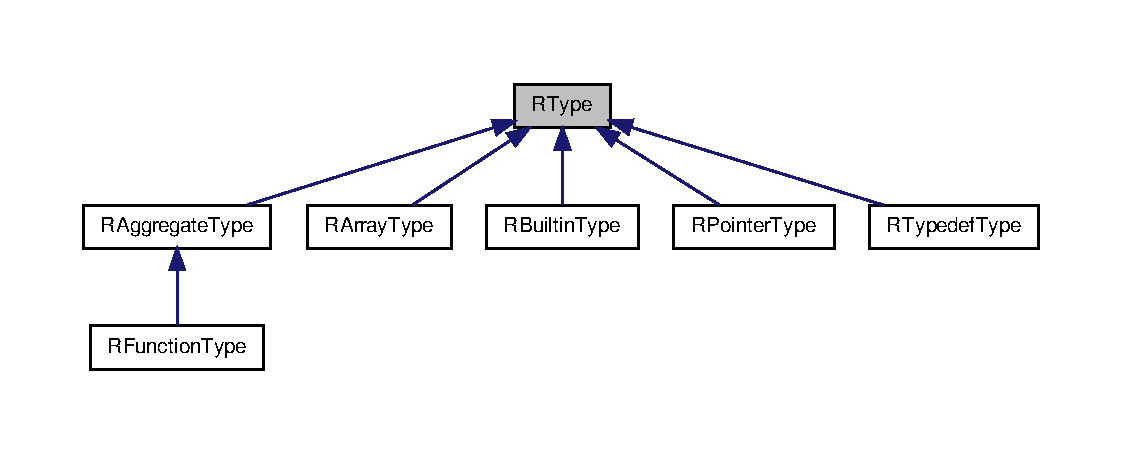
\includegraphics[width=350pt]{struct_r_type__inherit__graph}
\end{center}
\end{figure}
\subsubsection*{Public Member Functions}
\begin{DoxyCompactItemize}
\item 
\hyperlink{type_8h_a200873d33e0b46e4ae64e4bfd4f7ac9d}{R\-Type\-Id} \hyperlink{struct_r_type_a40ec26771acf938d1d4fd4968272bf43}{r\-\_\-type\-\_\-id} (\hyperlink{struct_r_type}{R\-Type} $\ast$type, G\-Error $\ast$$\ast$error)
\begin{DoxyCompactList}\small\item\em Get the type identifier of this type. \end{DoxyCompactList}\item 
\hyperlink{struct_r_string}{R\-String} $\ast$ \hyperlink{struct_r_type_a3693f92b73c76634fd1ea78521bb4947}{r\-\_\-type\-\_\-name} (\hyperlink{struct_r_type}{R\-Type} $\ast$type, G\-Error $\ast$$\ast$error)
\begin{DoxyCompactList}\small\item\em Get the name of this type. \end{DoxyCompactList}\item 
\hyperlink{struct_r_type}{R\-Type} $\ast$ \hyperlink{struct_r_type_a9796d0adc620247438780470f970d1fd}{r\-\_\-type\-\_\-ref} (\hyperlink{struct_r_type}{R\-Type} $\ast$type)
\begin{DoxyCompactList}\small\item\em Increase the reference count of this type. \end{DoxyCompactList}\item 
void \hyperlink{struct_r_type_abc901fe63aef5d4696ccd9bea136ea97}{r\-\_\-type\-\_\-unref} (\hyperlink{struct_r_type}{R\-Type} $\ast$type)
\begin{DoxyCompactList}\small\item\em Decrease the reference count of this. \end{DoxyCompactList}\item 
\hyperlink{struct_r_type}{R\-Type} $\ast$ \hyperlink{struct_r_type_ace0f37441c6f2d1a23f572269ac2d339}{r\-\_\-type\-\_\-pointer} (\hyperlink{struct_r_type}{R\-Type} $\ast$type, G\-Error $\ast$$\ast$error)
\begin{DoxyCompactList}\small\item\em Get an \hyperlink{struct_r_type}{R\-Type} representing a pointer to this type. \end{DoxyCompactList}\end{DoxyCompactItemize}


\subsubsection{Detailed Description}
An opaque struct representing a type. 

This type can be safely cast to it's sub-\/type which can be determined using \hyperlink{struct_r_type_a40ec26771acf938d1d4fd4968272bf43}{r\-\_\-type\-\_\-id()}. 

\subsubsection{Member Function Documentation}
\hypertarget{struct_r_type_a40ec26771acf938d1d4fd4968272bf43}{\index{R\-Type@{R\-Type}!r\-\_\-type\-\_\-id@{r\-\_\-type\-\_\-id}}
\index{r\-\_\-type\-\_\-id@{r\-\_\-type\-\_\-id}!RType@{R\-Type}}
\paragraph[{r\-\_\-type\-\_\-id}]{\setlength{\rightskip}{0pt plus 5cm}{\bf R\-Type\-Id} r\-\_\-type\-\_\-id (
\begin{DoxyParamCaption}
\item[{{\bf R\-Type} $\ast$}]{type, }
\item[{G\-Error $\ast$$\ast$}]{error}
\end{DoxyParamCaption}
)}}\label{struct_r_type_a40ec26771acf938d1d4fd4968272bf43}


Get the type identifier of this type. 

The R\-Type\-Id of this \hyperlink{struct_r_type}{R\-Type} represents the child type of this \hyperlink{struct_r_type}{R\-Type}, and can be safely cast into that child type.

\begin{DoxyReturn}{Returns}
the child type of this type. 
\end{DoxyReturn}

\begin{DoxyParams}[1]{Parameters}
\mbox{\tt in}  & {\em type} & the type to retrieve the type id of \\
\hline
\mbox{\tt out}  & {\em error} & see \hyperlink{errors_8h}{errors.\-h} \\
\hline
\end{DoxyParams}
\hypertarget{struct_r_type_a3693f92b73c76634fd1ea78521bb4947}{\index{R\-Type@{R\-Type}!r\-\_\-type\-\_\-name@{r\-\_\-type\-\_\-name}}
\index{r\-\_\-type\-\_\-name@{r\-\_\-type\-\_\-name}!RType@{R\-Type}}
\paragraph[{r\-\_\-type\-\_\-name}]{\setlength{\rightskip}{0pt plus 5cm}{\bf R\-String} $\ast$ r\-\_\-type\-\_\-name (
\begin{DoxyParamCaption}
\item[{{\bf R\-Type} $\ast$}]{type, }
\item[{G\-Error $\ast$$\ast$}]{error}
\end{DoxyParamCaption}
)}}\label{struct_r_type_a3693f92b73c76634fd1ea78521bb4947}


Get the name of this type. 

\begin{DoxyReturn}{Returns}
an \hyperlink{struct_r_string}{R\-String} containing the name of this type. 
\end{DoxyReturn}

\begin{DoxyParams}[1]{Parameters}
\mbox{\tt in}  & {\em type} & the type to retrieve the name of \\
\hline
\mbox{\tt out}  & {\em error} & see \hyperlink{errors_8h}{errors.\-h} \\
\hline
\end{DoxyParams}
\hypertarget{struct_r_type_ace0f37441c6f2d1a23f572269ac2d339}{\index{R\-Type@{R\-Type}!r\-\_\-type\-\_\-pointer@{r\-\_\-type\-\_\-pointer}}
\index{r\-\_\-type\-\_\-pointer@{r\-\_\-type\-\_\-pointer}!RType@{R\-Type}}
\paragraph[{r\-\_\-type\-\_\-pointer}]{\setlength{\rightskip}{0pt plus 5cm}{\bf R\-Type} $\ast$ r\-\_\-type\-\_\-pointer (
\begin{DoxyParamCaption}
\item[{{\bf R\-Type} $\ast$}]{type, }
\item[{G\-Error $\ast$$\ast$}]{error}
\end{DoxyParamCaption}
)}}\label{struct_r_type_ace0f37441c6f2d1a23f572269ac2d339}


Get an \hyperlink{struct_r_type}{R\-Type} representing a pointer to this type. 

\begin{DoxyReturn}{Returns}
An \hyperlink{struct_r_type}{R\-Type} representing a pointer to {\itshape type}. 
\end{DoxyReturn}

\begin{DoxyParams}[1]{Parameters}
\mbox{\tt in}  & {\em type} & the type to get a pointer to \\
\hline
\mbox{\tt out}  & {\em error} & see \hyperlink{errors_8h}{errors.\-h} \\
\hline
\end{DoxyParams}
\hypertarget{struct_r_type_a9796d0adc620247438780470f970d1fd}{\index{R\-Type@{R\-Type}!r\-\_\-type\-\_\-ref@{r\-\_\-type\-\_\-ref}}
\index{r\-\_\-type\-\_\-ref@{r\-\_\-type\-\_\-ref}!RType@{R\-Type}}
\paragraph[{r\-\_\-type\-\_\-ref}]{\setlength{\rightskip}{0pt plus 5cm}{\bf R\-Type} $\ast$ r\-\_\-type\-\_\-ref (
\begin{DoxyParamCaption}
\item[{{\bf R\-Type} $\ast$}]{type}
\end{DoxyParamCaption}
)}}\label{struct_r_type_a9796d0adc620247438780470f970d1fd}


Increase the reference count of this type. 

\begin{DoxyReturn}{Returns}
{\itshape type} 
\end{DoxyReturn}

\begin{DoxyParams}[1]{Parameters}
\mbox{\tt in}  & {\em type} & the type to increase the reference count of \\
\hline
\end{DoxyParams}
\hypertarget{struct_r_type_abc901fe63aef5d4696ccd9bea136ea97}{\index{R\-Type@{R\-Type}!r\-\_\-type\-\_\-unref@{r\-\_\-type\-\_\-unref}}
\index{r\-\_\-type\-\_\-unref@{r\-\_\-type\-\_\-unref}!RType@{R\-Type}}
\paragraph[{r\-\_\-type\-\_\-unref}]{\setlength{\rightskip}{0pt plus 5cm}void r\-\_\-type\-\_\-unref (
\begin{DoxyParamCaption}
\item[{{\bf R\-Type} $\ast$}]{type}
\end{DoxyParamCaption}
)}}\label{struct_r_type_abc901fe63aef5d4696ccd9bea136ea97}


Decrease the reference count of this. 

This \hyperlink{struct_r_type}{R\-Type} will be freed if the reference count drops to zero. 
\begin{DoxyParams}[1]{Parameters}
\mbox{\tt in}  & {\em type} & the type to decrease the reference count of \\
\hline
\end{DoxyParams}


The documentation for this struct was generated from the following file\-:\begin{DoxyCompactItemize}
\item 
ruminate/\hyperlink{type_8h}{type.\-h}\end{DoxyCompactItemize}

\hypertarget{struct_r_typedef_type}{\subsection{R\-Typedef\-Type Struct Reference}
\label{struct_r_typedef_type}\index{R\-Typedef\-Type@{R\-Typedef\-Type}}
}


An opaque struct representing a typedef'ed type.  




Inheritance diagram for R\-Typedef\-Type\-:\nopagebreak
\begin{figure}[H]
\begin{center}
\leavevmode
\includegraphics[width=160pt]{struct_r_typedef_type__inherit__graph}
\end{center}
\end{figure}
\subsubsection*{Public Member Functions}
\begin{DoxyCompactItemize}
\item 
\hyperlink{struct_r_type}{R\-Type} $\ast$ \hyperlink{struct_r_typedef_type_afa3538fc4df5050ba3df60547f36536c}{r\-\_\-typedef\-\_\-type\-\_\-canonical} (\hyperlink{struct_r_typedef_type}{R\-Typedef\-Type} $\ast$, G\-Error $\ast$$\ast$error)
\begin{DoxyCompactList}\small\item\em Get the canonical type of this type. \end{DoxyCompactList}\end{DoxyCompactItemize}


\subsubsection{Detailed Description}
An opaque struct representing a typedef'ed type. 

\subsubsection{Member Function Documentation}
\hypertarget{struct_r_typedef_type_afa3538fc4df5050ba3df60547f36536c}{\index{R\-Typedef\-Type@{R\-Typedef\-Type}!r\-\_\-typedef\-\_\-type\-\_\-canonical@{r\-\_\-typedef\-\_\-type\-\_\-canonical}}
\index{r\-\_\-typedef\-\_\-type\-\_\-canonical@{r\-\_\-typedef\-\_\-type\-\_\-canonical}!RTypedefType@{R\-Typedef\-Type}}
\paragraph[{r\-\_\-typedef\-\_\-type\-\_\-canonical}]{\setlength{\rightskip}{0pt plus 5cm}{\bf R\-Type} $\ast$ r\-\_\-typedef\-\_\-type\-\_\-canonical (
\begin{DoxyParamCaption}
\item[{{\bf R\-Typedef\-Type} $\ast$}]{, }
\item[{G\-Error $\ast$$\ast$}]{error}
\end{DoxyParamCaption}
)}}\label{struct_r_typedef_type_afa3538fc4df5050ba3df60547f36536c}


Get the canonical type of this type. 

A canonical type strips away all typedefs contained within this type.

For example with the following code, 
\begin{DoxyCode}
\textcolor{keyword}{typedef} \textcolor{keywordtype}{char} *String;
\textcolor{keyword}{typedef} String *StringArray;
\end{DoxyCode}
 calling \hyperlink{struct_r_typedef_type_afa3538fc4df5050ba3df60547f36536c}{r\-\_\-typedef\-\_\-type\-\_\-canonical()} on a \hyperlink{struct_r_typedef_type}{R\-Typedef\-Type} representing a {\ttfamily String\-Array} will return an \hyperlink{struct_r_type}{R\-Type} representing {\ttfamily char $\ast$$\ast$}.

\begin{DoxyRefDesc}{Todo}
\item[\hyperlink{todo__todo000008}{Todo}]Be able to single step through non-\/canonical types of an \hyperlink{struct_r_typedef_type}{R\-Typedef\-Type}. \end{DoxyRefDesc}
\begin{DoxyReturn}{Returns}
An \hyperlink{struct_r_type}{R\-Type} representing the canonical type of this \hyperlink{struct_r_typedef_type}{R\-Typedef\-Type}. 
\end{DoxyReturn}

\begin{DoxyParams}[1]{Parameters}
\mbox{\tt out}  & {\em error} & see \hyperlink{errors_8h}{errors.\-h} \\
\hline
\end{DoxyParams}


The documentation for this struct was generated from the following file\-:\begin{DoxyCompactItemize}
\item 
ruminate/typedef\-\_\-type.\-h\end{DoxyCompactItemize}

\hypertarget{struct_r_type_member}{\subsection{R\-Type\-Member Struct Reference}
\label{struct_r_type_member}\index{R\-Type\-Member@{R\-Type\-Member}}
}


An opaque struct representing a type member.  




Inheritance diagram for R\-Type\-Member\-:\nopagebreak
\begin{figure}[H]
\begin{center}
\leavevmode
\includegraphics[width=184pt]{struct_r_type_member__inherit__graph}
\end{center}
\end{figure}
\subsubsection*{Public Member Functions}
\begin{DoxyCompactItemize}
\item 
\hyperlink{type__member_8h_a57b8dacec0c2e6283f307c07aae6fb7f}{R\-Type\-Member\-Id} \hyperlink{struct_r_type_member_af0e43672c62600335cb0569266feb221}{r\-\_\-type\-\_\-member\-\_\-id} (\hyperlink{struct_r_type_member}{R\-Type\-Member} $\ast$member, G\-Error $\ast$$\ast$error)
\begin{DoxyCompactList}\small\item\em Get the type member id of this \hyperlink{struct_r_type_member}{R\-Type\-Member}. \end{DoxyCompactList}\item 
\hyperlink{struct_r_type}{R\-Type} $\ast$ \hyperlink{struct_r_type_member_a179498126b0805889ffcd113dfdff8f4}{r\-\_\-type\-\_\-member\-\_\-type} (\hyperlink{struct_r_type_member}{R\-Type\-Member} $\ast$member, G\-Error $\ast$$\ast$error)
\begin{DoxyCompactList}\small\item\em Get the type of this type member. \end{DoxyCompactList}\item 
ptrdiff\-\_\-t \hyperlink{struct_r_type_member_af192de4185914c999d0445d6a2f424d1}{r\-\_\-type\-\_\-member\-\_\-offset} (\hyperlink{struct_r_type_member}{R\-Type\-Member} $\ast$member, G\-Error $\ast$$\ast$error)
\begin{DoxyCompactList}\small\item\em Get the offset of this type member into it's container. \end{DoxyCompactList}\item 
\hyperlink{struct_r_type_member}{R\-Type\-Member} $\ast$ \hyperlink{struct_r_type_member_aa097c4e561c9db8aaf141d6d0a163310}{r\-\_\-type\-\_\-member\-\_\-ref} (\hyperlink{struct_r_type_member}{R\-Type\-Member} $\ast$member)
\begin{DoxyCompactList}\small\item\em Increment the reference count of this \hyperlink{struct_r_type_member}{R\-Type\-Member}. \end{DoxyCompactList}\item 
void \hyperlink{struct_r_type_member_aab80f39862cb60904fef002d635173f3}{r\-\_\-type\-\_\-member\-\_\-unref} (\hyperlink{struct_r_type_member}{R\-Type\-Member} $\ast$member)
\begin{DoxyCompactList}\small\item\em Decrement the reference count of this \hyperlink{struct_r_type_member}{R\-Type\-Member}. \end{DoxyCompactList}\end{DoxyCompactItemize}


\subsubsection{Detailed Description}
An opaque struct representing a type member. 

\subsubsection{Member Function Documentation}
\hypertarget{struct_r_type_member_af0e43672c62600335cb0569266feb221}{\index{R\-Type\-Member@{R\-Type\-Member}!r\-\_\-type\-\_\-member\-\_\-id@{r\-\_\-type\-\_\-member\-\_\-id}}
\index{r\-\_\-type\-\_\-member\-\_\-id@{r\-\_\-type\-\_\-member\-\_\-id}!RTypeMember@{R\-Type\-Member}}
\paragraph[{r\-\_\-type\-\_\-member\-\_\-id}]{\setlength{\rightskip}{0pt plus 5cm}{\bf R\-Type\-Member\-Id} r\-\_\-type\-\_\-member\-\_\-id (
\begin{DoxyParamCaption}
\item[{{\bf R\-Type\-Member} $\ast$}]{member, }
\item[{G\-Error $\ast$$\ast$}]{error}
\end{DoxyParamCaption}
)}}\label{struct_r_type_member_af0e43672c62600335cb0569266feb221}


Get the type member id of this \hyperlink{struct_r_type_member}{R\-Type\-Member}. 


\begin{DoxyParams}[1]{Parameters}
\mbox{\tt in}  & {\em member} & the type member to get the id of \\
\hline
\mbox{\tt out}  & {\em error} & see \hyperlink{errors_8h}{errors.\-h} \\
\hline
\end{DoxyParams}
\hypertarget{struct_r_type_member_af192de4185914c999d0445d6a2f424d1}{\index{R\-Type\-Member@{R\-Type\-Member}!r\-\_\-type\-\_\-member\-\_\-offset@{r\-\_\-type\-\_\-member\-\_\-offset}}
\index{r\-\_\-type\-\_\-member\-\_\-offset@{r\-\_\-type\-\_\-member\-\_\-offset}!RTypeMember@{R\-Type\-Member}}
\paragraph[{r\-\_\-type\-\_\-member\-\_\-offset}]{\setlength{\rightskip}{0pt plus 5cm}ptrdiff\-\_\-t r\-\_\-type\-\_\-member\-\_\-offset (
\begin{DoxyParamCaption}
\item[{{\bf R\-Type\-Member} $\ast$}]{member, }
\item[{G\-Error $\ast$$\ast$}]{error}
\end{DoxyParamCaption}
)}}\label{struct_r_type_member_af192de4185914c999d0445d6a2f424d1}


Get the offset of this type member into it's container. 

This is the number of bytes into this type member's container (either an \hyperlink{struct_r_array_type}{R\-Array\-Type}, or an \hyperlink{struct_r_aggregate_type}{R\-Aggregate\-Type}) that this member is located.

\begin{DoxySeeAlso}{See Also}
\hyperlink{struct_r_array_type}{R\-Array\-Type} 

\hyperlink{struct_r_aggregate_type}{R\-Aggregate\-Type} 
\end{DoxySeeAlso}

\begin{DoxyParams}[1]{Parameters}
\mbox{\tt in}  & {\em member} & the type member to get the offset of \\
\hline
\mbox{\tt out}  & {\em error} & see \hyperlink{errors_8h}{errors.\-h} \\
\hline
\end{DoxyParams}
\hypertarget{struct_r_type_member_aa097c4e561c9db8aaf141d6d0a163310}{\index{R\-Type\-Member@{R\-Type\-Member}!r\-\_\-type\-\_\-member\-\_\-ref@{r\-\_\-type\-\_\-member\-\_\-ref}}
\index{r\-\_\-type\-\_\-member\-\_\-ref@{r\-\_\-type\-\_\-member\-\_\-ref}!RTypeMember@{R\-Type\-Member}}
\paragraph[{r\-\_\-type\-\_\-member\-\_\-ref}]{\setlength{\rightskip}{0pt plus 5cm}{\bf R\-Type\-Member} $\ast$ r\-\_\-type\-\_\-member\-\_\-ref (
\begin{DoxyParamCaption}
\item[{{\bf R\-Type\-Member} $\ast$}]{member}
\end{DoxyParamCaption}
)}}\label{struct_r_type_member_aa097c4e561c9db8aaf141d6d0a163310}


Increment the reference count of this \hyperlink{struct_r_type_member}{R\-Type\-Member}. 


\begin{DoxyParams}[1]{Parameters}
\mbox{\tt in}  & {\em member} & the type member to increment the reference count of \\
\hline
\end{DoxyParams}
\hypertarget{struct_r_type_member_a179498126b0805889ffcd113dfdff8f4}{\index{R\-Type\-Member@{R\-Type\-Member}!r\-\_\-type\-\_\-member\-\_\-type@{r\-\_\-type\-\_\-member\-\_\-type}}
\index{r\-\_\-type\-\_\-member\-\_\-type@{r\-\_\-type\-\_\-member\-\_\-type}!RTypeMember@{R\-Type\-Member}}
\paragraph[{r\-\_\-type\-\_\-member\-\_\-type}]{\setlength{\rightskip}{0pt plus 5cm}{\bf R\-Type} $\ast$ r\-\_\-type\-\_\-member\-\_\-type (
\begin{DoxyParamCaption}
\item[{{\bf R\-Type\-Member} $\ast$}]{member, }
\item[{G\-Error $\ast$$\ast$}]{error}
\end{DoxyParamCaption}
)}}\label{struct_r_type_member_a179498126b0805889ffcd113dfdff8f4}


Get the type of this type member. 


\begin{DoxyParams}[1]{Parameters}
\mbox{\tt in}  & {\em member} & the type member to get the type of \\
\hline
\mbox{\tt out}  & {\em error} & see \hyperlink{errors_8h}{errors.\-h} \\
\hline
\end{DoxyParams}
\hypertarget{struct_r_type_member_aab80f39862cb60904fef002d635173f3}{\index{R\-Type\-Member@{R\-Type\-Member}!r\-\_\-type\-\_\-member\-\_\-unref@{r\-\_\-type\-\_\-member\-\_\-unref}}
\index{r\-\_\-type\-\_\-member\-\_\-unref@{r\-\_\-type\-\_\-member\-\_\-unref}!RTypeMember@{R\-Type\-Member}}
\paragraph[{r\-\_\-type\-\_\-member\-\_\-unref}]{\setlength{\rightskip}{0pt plus 5cm}void r\-\_\-type\-\_\-member\-\_\-unref (
\begin{DoxyParamCaption}
\item[{{\bf R\-Type\-Member} $\ast$}]{member}
\end{DoxyParamCaption}
)}}\label{struct_r_type_member_aab80f39862cb60904fef002d635173f3}


Decrement the reference count of this \hyperlink{struct_r_type_member}{R\-Type\-Member}. 

If the reference count reaches zero, this \hyperlink{struct_r_type_member}{R\-Type\-Member} will be freed. 
\begin{DoxyParams}[1]{Parameters}
\mbox{\tt in}  & {\em member} & the type member to decrement the reference count of \\
\hline
\end{DoxyParams}


The documentation for this struct was generated from the following file\-:\begin{DoxyCompactItemize}
\item 
ruminate/\hyperlink{type__member_8h}{type\-\_\-member.\-h}\end{DoxyCompactItemize}

\section{File Documentation}
\hypertarget{aggregate__member_8h}{\subsection{ruminate/aggregate\-\_\-member.h File Reference}
\label{aggregate__member_8h}\index{ruminate/aggregate\-\_\-member.\-h@{ruminate/aggregate\-\_\-member.\-h}}
}


Aggregate members.  


\subsubsection*{Enumerations}
\begin{DoxyCompactItemize}
\item 
enum \hyperlink{aggregate__member_8h_ae66a822b4bce9e1559fef33422de505c}{R\-Aggregate\-Member\-Id} \{ \\*
\hyperlink{aggregate__member_8h_ae66a822b4bce9e1559fef33422de505ca17343b5e162dcfc468d86be5c4035472}{R\-\_\-\-A\-G\-G\-R\-E\-G\-A\-T\-E\-\_\-\-M\-E\-M\-B\-E\-R\-\_\-\-B\-I\-T\-F\-I\-E\-L\-D}, 
\\*
\hyperlink{aggregate__member_8h_ae66a822b4bce9e1559fef33422de505ca595c194029b15546ab67947f7539e2a9}{R\-\_\-\-A\-G\-G\-R\-E\-G\-A\-T\-E\-\_\-\-M\-E\-M\-B\-E\-R\-\_\-\-E\-N\-U\-M}, 
\\*
\hyperlink{aggregate__member_8h_ae66a822b4bce9e1559fef33422de505cac2b6f8b0706160a7994cc2ca43432700}{R\-\_\-\-A\-G\-G\-R\-E\-G\-A\-T\-E\-\_\-\-M\-E\-M\-B\-E\-R\-\_\-\-O\-T\-H\-E\-R}
 \}
\begin{DoxyCompactList}\small\item\em An identifier denoting the real type of this \hyperlink{struct_r_aggregate_member}{R\-Aggregate\-Member}. \end{DoxyCompactList}\end{DoxyCompactItemize}


\subsubsection{Detailed Description}
Aggregate members. A \hyperlink{struct_r_aggregate_member}{R\-Aggregate\-Member} represents a member of an aggregate type.

\begin{DoxySeeAlso}{See Also}
\hyperlink{struct_r_aggregate_member}{R\-Aggregate\-Member} 

\hyperlink{struct_r_aggregate_type}{R\-Aggregate\-Type} 
\end{DoxySeeAlso}


\subsubsection{Enumeration Type Documentation}
\hypertarget{aggregate__member_8h_ae66a822b4bce9e1559fef33422de505c}{\index{aggregate\-\_\-member.\-h@{aggregate\-\_\-member.\-h}!R\-Aggregate\-Member\-Id@{R\-Aggregate\-Member\-Id}}
\index{R\-Aggregate\-Member\-Id@{R\-Aggregate\-Member\-Id}!aggregate_member.h@{aggregate\-\_\-member.\-h}}
\paragraph[{R\-Aggregate\-Member\-Id}]{\setlength{\rightskip}{0pt plus 5cm}enum {\bf R\-Aggregate\-Member\-Id}}}\label{aggregate__member_8h_ae66a822b4bce9e1559fef33422de505c}


An identifier denoting the real type of this \hyperlink{struct_r_aggregate_member}{R\-Aggregate\-Member}. 

This identifier can be retrieved using \hyperlink{struct_r_aggregate_member_a3d8b736967820633c1fcd3c91958cdea}{r\-\_\-aggregate\-\_\-member\-\_\-id()}. \begin{Desc}
\item[Enumerator]\par
\begin{description}
\index{R\-\_\-\-A\-G\-G\-R\-E\-G\-A\-T\-E\-\_\-\-M\-E\-M\-B\-E\-R\-\_\-\-B\-I\-T\-F\-I\-E\-L\-D@{R\-\_\-\-A\-G\-G\-R\-E\-G\-A\-T\-E\-\_\-\-M\-E\-M\-B\-E\-R\-\_\-\-B\-I\-T\-F\-I\-E\-L\-D}!aggregate\-\_\-member.\-h@{aggregate\-\_\-member.\-h}}\index{aggregate\-\_\-member.\-h@{aggregate\-\_\-member.\-h}!R\-\_\-\-A\-G\-G\-R\-E\-G\-A\-T\-E\-\_\-\-M\-E\-M\-B\-E\-R\-\_\-\-B\-I\-T\-F\-I\-E\-L\-D@{R\-\_\-\-A\-G\-G\-R\-E\-G\-A\-T\-E\-\_\-\-M\-E\-M\-B\-E\-R\-\_\-\-B\-I\-T\-F\-I\-E\-L\-D}}\item[{\em 
\hypertarget{aggregate__member_8h_ae66a822b4bce9e1559fef33422de505ca17343b5e162dcfc468d86be5c4035472}{R\-\_\-\-A\-G\-G\-R\-E\-G\-A\-T\-E\-\_\-\-M\-E\-M\-B\-E\-R\-\_\-\-B\-I\-T\-F\-I\-E\-L\-D}\label{aggregate__member_8h_ae66a822b4bce9e1559fef33422de505ca17343b5e162dcfc468d86be5c4035472}
}]a bitfield \index{R\-\_\-\-A\-G\-G\-R\-E\-G\-A\-T\-E\-\_\-\-M\-E\-M\-B\-E\-R\-\_\-\-E\-N\-U\-M@{R\-\_\-\-A\-G\-G\-R\-E\-G\-A\-T\-E\-\_\-\-M\-E\-M\-B\-E\-R\-\_\-\-E\-N\-U\-M}!aggregate\-\_\-member.\-h@{aggregate\-\_\-member.\-h}}\index{aggregate\-\_\-member.\-h@{aggregate\-\_\-member.\-h}!R\-\_\-\-A\-G\-G\-R\-E\-G\-A\-T\-E\-\_\-\-M\-E\-M\-B\-E\-R\-\_\-\-E\-N\-U\-M@{R\-\_\-\-A\-G\-G\-R\-E\-G\-A\-T\-E\-\_\-\-M\-E\-M\-B\-E\-R\-\_\-\-E\-N\-U\-M}}\item[{\em 
\hypertarget{aggregate__member_8h_ae66a822b4bce9e1559fef33422de505ca595c194029b15546ab67947f7539e2a9}{R\-\_\-\-A\-G\-G\-R\-E\-G\-A\-T\-E\-\_\-\-M\-E\-M\-B\-E\-R\-\_\-\-E\-N\-U\-M}\label{aggregate__member_8h_ae66a822b4bce9e1559fef33422de505ca595c194029b15546ab67947f7539e2a9}
}]an instance of \hyperlink{struct_r_enum_member}{R\-Enum\-Member} \begin{DoxySeeAlso}{See Also}
\hyperlink{struct_r_enum_member}{R\-Enum\-Member} 
\end{DoxySeeAlso}
\index{R\-\_\-\-A\-G\-G\-R\-E\-G\-A\-T\-E\-\_\-\-M\-E\-M\-B\-E\-R\-\_\-\-O\-T\-H\-E\-R@{R\-\_\-\-A\-G\-G\-R\-E\-G\-A\-T\-E\-\_\-\-M\-E\-M\-B\-E\-R\-\_\-\-O\-T\-H\-E\-R}!aggregate\-\_\-member.\-h@{aggregate\-\_\-member.\-h}}\index{aggregate\-\_\-member.\-h@{aggregate\-\_\-member.\-h}!R\-\_\-\-A\-G\-G\-R\-E\-G\-A\-T\-E\-\_\-\-M\-E\-M\-B\-E\-R\-\_\-\-O\-T\-H\-E\-R@{R\-\_\-\-A\-G\-G\-R\-E\-G\-A\-T\-E\-\_\-\-M\-E\-M\-B\-E\-R\-\_\-\-O\-T\-H\-E\-R}}\item[{\em 
\hypertarget{aggregate__member_8h_ae66a822b4bce9e1559fef33422de505cac2b6f8b0706160a7994cc2ca43432700}{R\-\_\-\-A\-G\-G\-R\-E\-G\-A\-T\-E\-\_\-\-M\-E\-M\-B\-E\-R\-\_\-\-O\-T\-H\-E\-R}\label{aggregate__member_8h_ae66a822b4bce9e1559fef33422de505cac2b6f8b0706160a7994cc2ca43432700}
}]a \char`\"{}normal\char`\"{} type (non enum-\/member nor bitfield) \end{description}
\end{Desc}

\hypertarget{aggregate__type_8h}{\subsection{ruminate/aggregate\-\_\-type.h File Reference}
\label{aggregate__type_8h}\index{ruminate/aggregate\-\_\-type.\-h@{ruminate/aggregate\-\_\-type.\-h}}
}


Aggregate types.  


\subsubsection*{Enumerations}
\begin{DoxyCompactItemize}
\item 
enum \hyperlink{aggregate__type_8h_ae208e3e28b5dcedb640f7f4b0581d61a}{R\-Aggregate\-Type\-Id} \{ \\*
\hyperlink{aggregate__type_8h_ae208e3e28b5dcedb640f7f4b0581d61aacbef5ea8a6646ea30c8af2618c98b77d}{R\-\_\-\-A\-G\-G\-R\-E\-G\-A\-T\-E\-\_\-\-T\-Y\-P\-E\-\_\-\-S\-T\-R\-U\-C\-T}, 
\\*
\hyperlink{aggregate__type_8h_ae208e3e28b5dcedb640f7f4b0581d61aa654a40297b4c4f6e363ae34596ab7e1a}{R\-\_\-\-A\-G\-G\-R\-E\-G\-A\-T\-E\-\_\-\-T\-Y\-P\-E\-\_\-\-U\-N\-I\-O\-N}, 
\\*
\hyperlink{aggregate__type_8h_ae208e3e28b5dcedb640f7f4b0581d61aa66dfd502a84ed416a4245ac248a1c344}{R\-\_\-\-A\-G\-G\-R\-E\-G\-A\-T\-E\-\_\-\-T\-Y\-P\-E\-\_\-\-E\-N\-U\-M}, 
\\*
\hyperlink{aggregate__type_8h_ae208e3e28b5dcedb640f7f4b0581d61aa145e538575fb274daa3e0f896be2c386}{R\-\_\-\-A\-G\-G\-R\-E\-G\-A\-T\-E\-\_\-\-T\-Y\-P\-E\-\_\-\-F\-U\-N\-C\-T\-I\-O\-N}, 
\\*
\hyperlink{aggregate__type_8h_ae208e3e28b5dcedb640f7f4b0581d61aa1a6412d28d7ed4fd0cddaad1bc3b84c4}{R\-\_\-\-A\-G\-G\-R\-E\-G\-A\-T\-E\-\_\-\-T\-Y\-P\-E\-\_\-\-U\-N\-K\-N\-O\-W\-N}
 \}
\begin{DoxyCompactList}\small\item\em An identifier denoting the child type of this \hyperlink{struct_r_aggregate_type}{R\-Aggregate\-Type}. \end{DoxyCompactList}\end{DoxyCompactItemize}


\subsubsection{Detailed Description}
Aggregate types. A \hyperlink{struct_r_aggregate_type}{R\-Aggregate\-Type} represents an aggregate type ({\ttfamily struct}, {\ttfamily union}, {\ttfamily enum} or {\ttfamily function})

\begin{DoxySeeAlso}{See Also}
\hyperlink{struct_r_aggregate_type}{R\-Aggregate\-Type} 
\end{DoxySeeAlso}


\subsubsection{Enumeration Type Documentation}
\hypertarget{aggregate__type_8h_ae208e3e28b5dcedb640f7f4b0581d61a}{\index{aggregate\-\_\-type.\-h@{aggregate\-\_\-type.\-h}!R\-Aggregate\-Type\-Id@{R\-Aggregate\-Type\-Id}}
\index{R\-Aggregate\-Type\-Id@{R\-Aggregate\-Type\-Id}!aggregate_type.h@{aggregate\-\_\-type.\-h}}
\paragraph[{R\-Aggregate\-Type\-Id}]{\setlength{\rightskip}{0pt plus 5cm}enum {\bf R\-Aggregate\-Type\-Id}}}\label{aggregate__type_8h_ae208e3e28b5dcedb640f7f4b0581d61a}


An identifier denoting the child type of this \hyperlink{struct_r_aggregate_type}{R\-Aggregate\-Type}. 

This identifier can be retrieved using \hyperlink{struct_r_aggregate_type_a3ad647b94dd87268b91e92f630b84726}{r\-\_\-aggregate\-\_\-type\-\_\-id()}. \begin{Desc}
\item[Enumerator]\par
\begin{description}
\index{R\-\_\-\-A\-G\-G\-R\-E\-G\-A\-T\-E\-\_\-\-T\-Y\-P\-E\-\_\-\-S\-T\-R\-U\-C\-T@{R\-\_\-\-A\-G\-G\-R\-E\-G\-A\-T\-E\-\_\-\-T\-Y\-P\-E\-\_\-\-S\-T\-R\-U\-C\-T}!aggregate\-\_\-type.\-h@{aggregate\-\_\-type.\-h}}\index{aggregate\-\_\-type.\-h@{aggregate\-\_\-type.\-h}!R\-\_\-\-A\-G\-G\-R\-E\-G\-A\-T\-E\-\_\-\-T\-Y\-P\-E\-\_\-\-S\-T\-R\-U\-C\-T@{R\-\_\-\-A\-G\-G\-R\-E\-G\-A\-T\-E\-\_\-\-T\-Y\-P\-E\-\_\-\-S\-T\-R\-U\-C\-T}}\item[{\em 
\hypertarget{aggregate__type_8h_ae208e3e28b5dcedb640f7f4b0581d61aacbef5ea8a6646ea30c8af2618c98b77d}{R\-\_\-\-A\-G\-G\-R\-E\-G\-A\-T\-E\-\_\-\-T\-Y\-P\-E\-\_\-\-S\-T\-R\-U\-C\-T}\label{aggregate__type_8h_ae208e3e28b5dcedb640f7f4b0581d61aacbef5ea8a6646ea30c8af2618c98b77d}
}]a {\ttfamily struct} \index{R\-\_\-\-A\-G\-G\-R\-E\-G\-A\-T\-E\-\_\-\-T\-Y\-P\-E\-\_\-\-U\-N\-I\-O\-N@{R\-\_\-\-A\-G\-G\-R\-E\-G\-A\-T\-E\-\_\-\-T\-Y\-P\-E\-\_\-\-U\-N\-I\-O\-N}!aggregate\-\_\-type.\-h@{aggregate\-\_\-type.\-h}}\index{aggregate\-\_\-type.\-h@{aggregate\-\_\-type.\-h}!R\-\_\-\-A\-G\-G\-R\-E\-G\-A\-T\-E\-\_\-\-T\-Y\-P\-E\-\_\-\-U\-N\-I\-O\-N@{R\-\_\-\-A\-G\-G\-R\-E\-G\-A\-T\-E\-\_\-\-T\-Y\-P\-E\-\_\-\-U\-N\-I\-O\-N}}\item[{\em 
\hypertarget{aggregate__type_8h_ae208e3e28b5dcedb640f7f4b0581d61aa654a40297b4c4f6e363ae34596ab7e1a}{R\-\_\-\-A\-G\-G\-R\-E\-G\-A\-T\-E\-\_\-\-T\-Y\-P\-E\-\_\-\-U\-N\-I\-O\-N}\label{aggregate__type_8h_ae208e3e28b5dcedb640f7f4b0581d61aa654a40297b4c4f6e363ae34596ab7e1a}
}]a {\ttfamily union} \index{R\-\_\-\-A\-G\-G\-R\-E\-G\-A\-T\-E\-\_\-\-T\-Y\-P\-E\-\_\-\-E\-N\-U\-M@{R\-\_\-\-A\-G\-G\-R\-E\-G\-A\-T\-E\-\_\-\-T\-Y\-P\-E\-\_\-\-E\-N\-U\-M}!aggregate\-\_\-type.\-h@{aggregate\-\_\-type.\-h}}\index{aggregate\-\_\-type.\-h@{aggregate\-\_\-type.\-h}!R\-\_\-\-A\-G\-G\-R\-E\-G\-A\-T\-E\-\_\-\-T\-Y\-P\-E\-\_\-\-E\-N\-U\-M@{R\-\_\-\-A\-G\-G\-R\-E\-G\-A\-T\-E\-\_\-\-T\-Y\-P\-E\-\_\-\-E\-N\-U\-M}}\item[{\em 
\hypertarget{aggregate__type_8h_ae208e3e28b5dcedb640f7f4b0581d61aa66dfd502a84ed416a4245ac248a1c344}{R\-\_\-\-A\-G\-G\-R\-E\-G\-A\-T\-E\-\_\-\-T\-Y\-P\-E\-\_\-\-E\-N\-U\-M}\label{aggregate__type_8h_ae208e3e28b5dcedb640f7f4b0581d61aa66dfd502a84ed416a4245ac248a1c344}
}]an {\ttfamily enum} \index{R\-\_\-\-A\-G\-G\-R\-E\-G\-A\-T\-E\-\_\-\-T\-Y\-P\-E\-\_\-\-F\-U\-N\-C\-T\-I\-O\-N@{R\-\_\-\-A\-G\-G\-R\-E\-G\-A\-T\-E\-\_\-\-T\-Y\-P\-E\-\_\-\-F\-U\-N\-C\-T\-I\-O\-N}!aggregate\-\_\-type.\-h@{aggregate\-\_\-type.\-h}}\index{aggregate\-\_\-type.\-h@{aggregate\-\_\-type.\-h}!R\-\_\-\-A\-G\-G\-R\-E\-G\-A\-T\-E\-\_\-\-T\-Y\-P\-E\-\_\-\-F\-U\-N\-C\-T\-I\-O\-N@{R\-\_\-\-A\-G\-G\-R\-E\-G\-A\-T\-E\-\_\-\-T\-Y\-P\-E\-\_\-\-F\-U\-N\-C\-T\-I\-O\-N}}\item[{\em 
\hypertarget{aggregate__type_8h_ae208e3e28b5dcedb640f7f4b0581d61aa145e538575fb274daa3e0f896be2c386}{R\-\_\-\-A\-G\-G\-R\-E\-G\-A\-T\-E\-\_\-\-T\-Y\-P\-E\-\_\-\-F\-U\-N\-C\-T\-I\-O\-N}\label{aggregate__type_8h_ae208e3e28b5dcedb640f7f4b0581d61aa145e538575fb274daa3e0f896be2c386}
}]a function type \begin{DoxySeeAlso}{See Also}
\hyperlink{struct_r_function_type}{R\-Function\-Type} 
\end{DoxySeeAlso}
\index{R\-\_\-\-A\-G\-G\-R\-E\-G\-A\-T\-E\-\_\-\-T\-Y\-P\-E\-\_\-\-U\-N\-K\-N\-O\-W\-N@{R\-\_\-\-A\-G\-G\-R\-E\-G\-A\-T\-E\-\_\-\-T\-Y\-P\-E\-\_\-\-U\-N\-K\-N\-O\-W\-N}!aggregate\-\_\-type.\-h@{aggregate\-\_\-type.\-h}}\index{aggregate\-\_\-type.\-h@{aggregate\-\_\-type.\-h}!R\-\_\-\-A\-G\-G\-R\-E\-G\-A\-T\-E\-\_\-\-T\-Y\-P\-E\-\_\-\-U\-N\-K\-N\-O\-W\-N@{R\-\_\-\-A\-G\-G\-R\-E\-G\-A\-T\-E\-\_\-\-T\-Y\-P\-E\-\_\-\-U\-N\-K\-N\-O\-W\-N}}\item[{\em 
\hypertarget{aggregate__type_8h_ae208e3e28b5dcedb640f7f4b0581d61aa1a6412d28d7ed4fd0cddaad1bc3b84c4}{R\-\_\-\-A\-G\-G\-R\-E\-G\-A\-T\-E\-\_\-\-T\-Y\-P\-E\-\_\-\-U\-N\-K\-N\-O\-W\-N}\label{aggregate__type_8h_ae208e3e28b5dcedb640f7f4b0581d61aa1a6412d28d7ed4fd0cddaad1bc3b84c4}
}]an unknown type \end{description}
\end{Desc}

\hypertarget{builtin__type_8h}{\subsection{ruminate/builtin\-\_\-type.h File Reference}
\label{builtin__type_8h}\index{ruminate/builtin\-\_\-type.\-h@{ruminate/builtin\-\_\-type.\-h}}
}


Built-\/in types.  


\subsubsection*{Enumerations}
\begin{DoxyCompactItemize}
\item 
enum \hyperlink{builtin__type_8h_a245d1724f16dd995c090e6666722c80c}{R\-Builtin\-Type\-Id} \{ \\*
\hyperlink{builtin__type_8h_a245d1724f16dd995c090e6666722c80cadfca796547cdc00ccfdbe77706074951}{R\-\_\-\-B\-U\-I\-L\-T\-I\-N\-\_\-\-T\-Y\-P\-E\-\_\-\-I\-N\-T}, 
\\*
\hyperlink{builtin__type_8h_a245d1724f16dd995c090e6666722c80ca36faa0523ded95ededf69e188b3396ba}{R\-\_\-\-B\-U\-I\-L\-T\-I\-N\-\_\-\-T\-Y\-P\-E\-\_\-\-L\-O\-N\-G}, 
\\*
\hyperlink{builtin__type_8h_a245d1724f16dd995c090e6666722c80cae875979c13faa722ea7ea3f7d7ec0d5b}{R\-\_\-\-B\-U\-I\-L\-T\-I\-N\-\_\-\-T\-Y\-P\-E\-\_\-\-D\-O\-U\-B\-L\-E}, 
\\*
\hyperlink{builtin__type_8h_a245d1724f16dd995c090e6666722c80caf128c571162a77fe48a93371a43f8013}{R\-\_\-\-B\-U\-I\-L\-T\-I\-N\-\_\-\-T\-Y\-P\-E\-\_\-\-S\-H\-O\-R\-T}, 
\\*
\hyperlink{builtin__type_8h_a245d1724f16dd995c090e6666722c80ca522e3cde81f0f3bd98ac9eb3f302267a}{R\-\_\-\-B\-U\-I\-L\-T\-I\-N\-\_\-\-T\-Y\-P\-E\-\_\-\-C\-H\-A\-R}, 
\\*
\hyperlink{builtin__type_8h_a245d1724f16dd995c090e6666722c80ca27dd26ba34fa61cfca7a5c9192337d5f}{R\-\_\-\-B\-U\-I\-L\-T\-I\-N\-\_\-\-T\-Y\-P\-E\-\_\-\-V\-O\-I\-D}, 
\\*
\hyperlink{builtin__type_8h_a245d1724f16dd995c090e6666722c80caa2f78ebf380cc94ab7c3b73eaa30e3d1}{R\-\_\-\-B\-U\-I\-L\-T\-I\-N\-\_\-\-T\-Y\-P\-E\-\_\-\-B\-O\-O\-L}, 
\\*
\hyperlink{builtin__type_8h_a245d1724f16dd995c090e6666722c80cac6acf9f77979e6021dc2c023d00a0431}{R\-\_\-\-B\-U\-I\-L\-T\-I\-N\-\_\-\-T\-Y\-P\-E\-\_\-\-U\-N\-K\-N\-O\-W\-N}
 \}
\begin{DoxyCompactList}\small\item\em An identifier denoting the real type of this \hyperlink{struct_r_builtin_type}{R\-Builtin\-Type}. \end{DoxyCompactList}\end{DoxyCompactItemize}


\subsubsection{Detailed Description}
Built-\/in types. A R\-Buintin\-Type represents a built-\/in type ({\ttfamily int}, {\ttfamily double}, etc.)

\begin{DoxySeeAlso}{See Also}
\hyperlink{struct_r_builtin_type}{R\-Builtin\-Type} 
\end{DoxySeeAlso}


\subsubsection{Enumeration Type Documentation}
\hypertarget{builtin__type_8h_a245d1724f16dd995c090e6666722c80c}{\index{builtin\-\_\-type.\-h@{builtin\-\_\-type.\-h}!R\-Builtin\-Type\-Id@{R\-Builtin\-Type\-Id}}
\index{R\-Builtin\-Type\-Id@{R\-Builtin\-Type\-Id}!builtin_type.h@{builtin\-\_\-type.\-h}}
\paragraph[{R\-Builtin\-Type\-Id}]{\setlength{\rightskip}{0pt plus 5cm}enum {\bf R\-Builtin\-Type\-Id}}}\label{builtin__type_8h_a245d1724f16dd995c090e6666722c80c}


An identifier denoting the real type of this \hyperlink{struct_r_builtin_type}{R\-Builtin\-Type}. 

This identifier can be retrieved using \hyperlink{struct_r_builtin_type_afaf0b8970072c1587ebc7936eaccbcee}{r\-\_\-builtin\-\_\-type\-\_\-id()}. \begin{Desc}
\item[Enumerator]\par
\begin{description}
\index{R\-\_\-\-B\-U\-I\-L\-T\-I\-N\-\_\-\-T\-Y\-P\-E\-\_\-\-I\-N\-T@{R\-\_\-\-B\-U\-I\-L\-T\-I\-N\-\_\-\-T\-Y\-P\-E\-\_\-\-I\-N\-T}!builtin\-\_\-type.\-h@{builtin\-\_\-type.\-h}}\index{builtin\-\_\-type.\-h@{builtin\-\_\-type.\-h}!R\-\_\-\-B\-U\-I\-L\-T\-I\-N\-\_\-\-T\-Y\-P\-E\-\_\-\-I\-N\-T@{R\-\_\-\-B\-U\-I\-L\-T\-I\-N\-\_\-\-T\-Y\-P\-E\-\_\-\-I\-N\-T}}\item[{\em 
\hypertarget{builtin__type_8h_a245d1724f16dd995c090e6666722c80cadfca796547cdc00ccfdbe77706074951}{R\-\_\-\-B\-U\-I\-L\-T\-I\-N\-\_\-\-T\-Y\-P\-E\-\_\-\-I\-N\-T}\label{builtin__type_8h_a245d1724f16dd995c090e6666722c80cadfca796547cdc00ccfdbe77706074951}
}]an int \index{R\-\_\-\-B\-U\-I\-L\-T\-I\-N\-\_\-\-T\-Y\-P\-E\-\_\-\-L\-O\-N\-G@{R\-\_\-\-B\-U\-I\-L\-T\-I\-N\-\_\-\-T\-Y\-P\-E\-\_\-\-L\-O\-N\-G}!builtin\-\_\-type.\-h@{builtin\-\_\-type.\-h}}\index{builtin\-\_\-type.\-h@{builtin\-\_\-type.\-h}!R\-\_\-\-B\-U\-I\-L\-T\-I\-N\-\_\-\-T\-Y\-P\-E\-\_\-\-L\-O\-N\-G@{R\-\_\-\-B\-U\-I\-L\-T\-I\-N\-\_\-\-T\-Y\-P\-E\-\_\-\-L\-O\-N\-G}}\item[{\em 
\hypertarget{builtin__type_8h_a245d1724f16dd995c090e6666722c80ca36faa0523ded95ededf69e188b3396ba}{R\-\_\-\-B\-U\-I\-L\-T\-I\-N\-\_\-\-T\-Y\-P\-E\-\_\-\-L\-O\-N\-G}\label{builtin__type_8h_a245d1724f16dd995c090e6666722c80ca36faa0523ded95ededf69e188b3396ba}
}]a long \index{R\-\_\-\-B\-U\-I\-L\-T\-I\-N\-\_\-\-T\-Y\-P\-E\-\_\-\-D\-O\-U\-B\-L\-E@{R\-\_\-\-B\-U\-I\-L\-T\-I\-N\-\_\-\-T\-Y\-P\-E\-\_\-\-D\-O\-U\-B\-L\-E}!builtin\-\_\-type.\-h@{builtin\-\_\-type.\-h}}\index{builtin\-\_\-type.\-h@{builtin\-\_\-type.\-h}!R\-\_\-\-B\-U\-I\-L\-T\-I\-N\-\_\-\-T\-Y\-P\-E\-\_\-\-D\-O\-U\-B\-L\-E@{R\-\_\-\-B\-U\-I\-L\-T\-I\-N\-\_\-\-T\-Y\-P\-E\-\_\-\-D\-O\-U\-B\-L\-E}}\item[{\em 
\hypertarget{builtin__type_8h_a245d1724f16dd995c090e6666722c80cae875979c13faa722ea7ea3f7d7ec0d5b}{R\-\_\-\-B\-U\-I\-L\-T\-I\-N\-\_\-\-T\-Y\-P\-E\-\_\-\-D\-O\-U\-B\-L\-E}\label{builtin__type_8h_a245d1724f16dd995c090e6666722c80cae875979c13faa722ea7ea3f7d7ec0d5b}
}]a double \index{R\-\_\-\-B\-U\-I\-L\-T\-I\-N\-\_\-\-T\-Y\-P\-E\-\_\-\-S\-H\-O\-R\-T@{R\-\_\-\-B\-U\-I\-L\-T\-I\-N\-\_\-\-T\-Y\-P\-E\-\_\-\-S\-H\-O\-R\-T}!builtin\-\_\-type.\-h@{builtin\-\_\-type.\-h}}\index{builtin\-\_\-type.\-h@{builtin\-\_\-type.\-h}!R\-\_\-\-B\-U\-I\-L\-T\-I\-N\-\_\-\-T\-Y\-P\-E\-\_\-\-S\-H\-O\-R\-T@{R\-\_\-\-B\-U\-I\-L\-T\-I\-N\-\_\-\-T\-Y\-P\-E\-\_\-\-S\-H\-O\-R\-T}}\item[{\em 
\hypertarget{builtin__type_8h_a245d1724f16dd995c090e6666722c80caf128c571162a77fe48a93371a43f8013}{R\-\_\-\-B\-U\-I\-L\-T\-I\-N\-\_\-\-T\-Y\-P\-E\-\_\-\-S\-H\-O\-R\-T}\label{builtin__type_8h_a245d1724f16dd995c090e6666722c80caf128c571162a77fe48a93371a43f8013}
}]a short \index{R\-\_\-\-B\-U\-I\-L\-T\-I\-N\-\_\-\-T\-Y\-P\-E\-\_\-\-C\-H\-A\-R@{R\-\_\-\-B\-U\-I\-L\-T\-I\-N\-\_\-\-T\-Y\-P\-E\-\_\-\-C\-H\-A\-R}!builtin\-\_\-type.\-h@{builtin\-\_\-type.\-h}}\index{builtin\-\_\-type.\-h@{builtin\-\_\-type.\-h}!R\-\_\-\-B\-U\-I\-L\-T\-I\-N\-\_\-\-T\-Y\-P\-E\-\_\-\-C\-H\-A\-R@{R\-\_\-\-B\-U\-I\-L\-T\-I\-N\-\_\-\-T\-Y\-P\-E\-\_\-\-C\-H\-A\-R}}\item[{\em 
\hypertarget{builtin__type_8h_a245d1724f16dd995c090e6666722c80ca522e3cde81f0f3bd98ac9eb3f302267a}{R\-\_\-\-B\-U\-I\-L\-T\-I\-N\-\_\-\-T\-Y\-P\-E\-\_\-\-C\-H\-A\-R}\label{builtin__type_8h_a245d1724f16dd995c090e6666722c80ca522e3cde81f0f3bd98ac9eb3f302267a}
}]a char \index{R\-\_\-\-B\-U\-I\-L\-T\-I\-N\-\_\-\-T\-Y\-P\-E\-\_\-\-V\-O\-I\-D@{R\-\_\-\-B\-U\-I\-L\-T\-I\-N\-\_\-\-T\-Y\-P\-E\-\_\-\-V\-O\-I\-D}!builtin\-\_\-type.\-h@{builtin\-\_\-type.\-h}}\index{builtin\-\_\-type.\-h@{builtin\-\_\-type.\-h}!R\-\_\-\-B\-U\-I\-L\-T\-I\-N\-\_\-\-T\-Y\-P\-E\-\_\-\-V\-O\-I\-D@{R\-\_\-\-B\-U\-I\-L\-T\-I\-N\-\_\-\-T\-Y\-P\-E\-\_\-\-V\-O\-I\-D}}\item[{\em 
\hypertarget{builtin__type_8h_a245d1724f16dd995c090e6666722c80ca27dd26ba34fa61cfca7a5c9192337d5f}{R\-\_\-\-B\-U\-I\-L\-T\-I\-N\-\_\-\-T\-Y\-P\-E\-\_\-\-V\-O\-I\-D}\label{builtin__type_8h_a245d1724f16dd995c090e6666722c80ca27dd26ba34fa61cfca7a5c9192337d5f}
}]the void type \index{R\-\_\-\-B\-U\-I\-L\-T\-I\-N\-\_\-\-T\-Y\-P\-E\-\_\-\-B\-O\-O\-L@{R\-\_\-\-B\-U\-I\-L\-T\-I\-N\-\_\-\-T\-Y\-P\-E\-\_\-\-B\-O\-O\-L}!builtin\-\_\-type.\-h@{builtin\-\_\-type.\-h}}\index{builtin\-\_\-type.\-h@{builtin\-\_\-type.\-h}!R\-\_\-\-B\-U\-I\-L\-T\-I\-N\-\_\-\-T\-Y\-P\-E\-\_\-\-B\-O\-O\-L@{R\-\_\-\-B\-U\-I\-L\-T\-I\-N\-\_\-\-T\-Y\-P\-E\-\_\-\-B\-O\-O\-L}}\item[{\em 
\hypertarget{builtin__type_8h_a245d1724f16dd995c090e6666722c80caa2f78ebf380cc94ab7c3b73eaa30e3d1}{R\-\_\-\-B\-U\-I\-L\-T\-I\-N\-\_\-\-T\-Y\-P\-E\-\_\-\-B\-O\-O\-L}\label{builtin__type_8h_a245d1724f16dd995c090e6666722c80caa2f78ebf380cc94ab7c3b73eaa30e3d1}
}]a bool \index{R\-\_\-\-B\-U\-I\-L\-T\-I\-N\-\_\-\-T\-Y\-P\-E\-\_\-\-U\-N\-K\-N\-O\-W\-N@{R\-\_\-\-B\-U\-I\-L\-T\-I\-N\-\_\-\-T\-Y\-P\-E\-\_\-\-U\-N\-K\-N\-O\-W\-N}!builtin\-\_\-type.\-h@{builtin\-\_\-type.\-h}}\index{builtin\-\_\-type.\-h@{builtin\-\_\-type.\-h}!R\-\_\-\-B\-U\-I\-L\-T\-I\-N\-\_\-\-T\-Y\-P\-E\-\_\-\-U\-N\-K\-N\-O\-W\-N@{R\-\_\-\-B\-U\-I\-L\-T\-I\-N\-\_\-\-T\-Y\-P\-E\-\_\-\-U\-N\-K\-N\-O\-W\-N}}\item[{\em 
\hypertarget{builtin__type_8h_a245d1724f16dd995c090e6666722c80cac6acf9f77979e6021dc2c023d00a0431}{R\-\_\-\-B\-U\-I\-L\-T\-I\-N\-\_\-\-T\-Y\-P\-E\-\_\-\-U\-N\-K\-N\-O\-W\-N}\label{builtin__type_8h_a245d1724f16dd995c090e6666722c80cac6acf9f77979e6021dc2c023d00a0431}
}]an unknown type \end{description}
\end{Desc}

\hypertarget{errors_8h}{\subsection{ruminate/errors.h File Reference}
\label{errors_8h}\index{ruminate/errors.\-h@{ruminate/errors.\-h}}
}


Error handling facilities.  


\subsubsection*{Macros}
\begin{DoxyCompactItemize}
\item 
\#define \hyperlink{errors_8h_a4485d35c67e4845c47a7fdd873cc20d5}{R\-U\-M\-I\-N\-A\-T\-E\-\_\-\-E\-R\-R\-O\-R}
\begin{DoxyCompactList}\small\item\em The error quark representing errors produced by this library. \end{DoxyCompactList}\item 
\#define \hyperlink{errors_8h_a2056c4b5b8b5761d8fe7776f09247405}{R\-U\-M\-I\-N\-A\-T\-E\-\_\-\-E\-R\-R\-N\-O\-\_\-\-E\-R\-R\-O\-R}
\begin{DoxyCompactList}\small\item\em The error quark representing errors produced by the standard C library. \end{DoxyCompactList}\end{DoxyCompactItemize}
\subsubsection*{Enumerations}
\begin{DoxyCompactItemize}
\item 
enum \hyperlink{errors_8h_a0bff341b89fef12fd9562ce9a23f8f54}{Ruminate\-Error} \{ \\*
{\bfseries R\-U\-M\-I\-N\-A\-T\-E\-\_\-\-E\-R\-R\-O\-R\-\_\-\-S\-B\-\_\-\-I\-N\-V\-A\-L\-I\-D}, 
\\*
{\bfseries R\-U\-M\-I\-N\-A\-T\-E\-\_\-\-E\-R\-R\-O\-R\-\_\-\-L\-L\-D\-B\-\_\-\-E\-R\-R\-O\-R}, 
\\*
{\bfseries R\-U\-M\-I\-N\-A\-T\-E\-\_\-\-E\-R\-R\-O\-R\-\_\-\-R\-A\-N\-G\-E}, 
\\*
{\bfseries R\-U\-M\-I\-N\-A\-T\-E\-\_\-\-E\-R\-R\-O\-R\-\_\-\-N\-O\-\_\-\-P\-R\-I\-M\-I\-T\-I\-V\-E\-\_\-\-T\-Y\-P\-E}, 
\\*
{\bfseries R\-U\-M\-I\-N\-A\-T\-E\-\_\-\-E\-R\-R\-O\-R\-\_\-\-I\-N\-V\-A\-L\-I\-D\-\_\-\-T\-Y\-P\-E}, 
\\*
{\bfseries R\-U\-M\-I\-N\-A\-T\-E\-\_\-\-E\-R\-R\-O\-R\-\_\-\-I\-N\-C\-O\-M\-P\-L\-E\-T\-E\-\_\-\-T\-Y\-P\-E}, 
\\*
{\bfseries R\-U\-M\-I\-N\-A\-T\-E\-\_\-\-E\-R\-R\-O\-R\-\_\-\-I\-C\-E}, 
\\*
{\bfseries R\-U\-M\-I\-N\-A\-T\-E\-\_\-\-E\-R\-R\-O\-R\-\_\-\-S\-T\-D\-L\-I\-B}, 
\\*
{\bfseries R\-U\-M\-I\-N\-A\-T\-E\-\_\-\-E\-R\-R\-O\-R\-\_\-\-S\-H\-O\-R\-T\-\_\-\-R\-E\-A\-D}, 
\\*
{\bfseries R\-U\-M\-I\-N\-A\-T\-E\-\_\-\-E\-R\-R\-O\-R\-\_\-\-N\-O\-\_\-\-P\-R\-G\-N\-A\-M\-E}, 
\\*
{\bfseries R\-U\-M\-I\-N\-A\-T\-E\-\_\-\-E\-R\-R\-O\-R\-\_\-\-U\-N\-I\-M\-P\-L\-E\-M\-E\-N\-T\-E\-D}, 
\\*
{\bfseries R\-U\-M\-I\-N\-A\-T\-E\-\_\-\-E\-R\-R\-O\-R\-\_\-\-U\-N\-S\-P\-E\-C}
 \}
\begin{DoxyCompactList}\small\item\em The various errors produced by ruminate. \end{DoxyCompactList}\end{DoxyCompactItemize}


\subsubsection{Detailed Description}
Error handling facilities. Every function which takes as an argument a {\ttfamily G\-Error $\ast$$\ast$} reports errors through this pointer.

In brief, pass {\ttfamily N\-U\-L\-L} as the {\ttfamily G\-Error $\ast$$\ast$} argument to functions or pass a pointer to a {\ttfamily N\-U\-L\-L} {\ttfamily G\-Error $\ast$} to recieve a {\ttfamily G\-Error} when an error occurs.

\begin{DoxySeeAlso}{See Also}
\href{https://developer.gnome.org/glib/2.34/glib-Error-Reporting.html}{\tt G\-Error} 
\end{DoxySeeAlso}


\subsubsection{Macro Definition Documentation}
\hypertarget{errors_8h_a2056c4b5b8b5761d8fe7776f09247405}{\index{errors.\-h@{errors.\-h}!R\-U\-M\-I\-N\-A\-T\-E\-\_\-\-E\-R\-R\-N\-O\-\_\-\-E\-R\-R\-O\-R@{R\-U\-M\-I\-N\-A\-T\-E\-\_\-\-E\-R\-R\-N\-O\-\_\-\-E\-R\-R\-O\-R}}
\index{R\-U\-M\-I\-N\-A\-T\-E\-\_\-\-E\-R\-R\-N\-O\-\_\-\-E\-R\-R\-O\-R@{R\-U\-M\-I\-N\-A\-T\-E\-\_\-\-E\-R\-R\-N\-O\-\_\-\-E\-R\-R\-O\-R}!errors.h@{errors.\-h}}
\paragraph[{R\-U\-M\-I\-N\-A\-T\-E\-\_\-\-E\-R\-R\-N\-O\-\_\-\-E\-R\-R\-O\-R}]{\setlength{\rightskip}{0pt plus 5cm}\#define R\-U\-M\-I\-N\-A\-T\-E\-\_\-\-E\-R\-R\-N\-O\-\_\-\-E\-R\-R\-O\-R}}\label{errors_8h_a2056c4b5b8b5761d8fe7776f09247405}


The error quark representing errors produced by the standard C library. 

This quark will be placed in the {\ttfamily domain} field of a {\ttfamily G\-Error} produced when an error occurrs.

\begin{DoxySeeAlso}{See Also}
\href{https://developer.gnome.org/glib/2.34/glib-Quarks.html}{\tt G\-Quark} 
\end{DoxySeeAlso}
\hypertarget{errors_8h_a4485d35c67e4845c47a7fdd873cc20d5}{\index{errors.\-h@{errors.\-h}!R\-U\-M\-I\-N\-A\-T\-E\-\_\-\-E\-R\-R\-O\-R@{R\-U\-M\-I\-N\-A\-T\-E\-\_\-\-E\-R\-R\-O\-R}}
\index{R\-U\-M\-I\-N\-A\-T\-E\-\_\-\-E\-R\-R\-O\-R@{R\-U\-M\-I\-N\-A\-T\-E\-\_\-\-E\-R\-R\-O\-R}!errors.h@{errors.\-h}}
\paragraph[{R\-U\-M\-I\-N\-A\-T\-E\-\_\-\-E\-R\-R\-O\-R}]{\setlength{\rightskip}{0pt plus 5cm}\#define R\-U\-M\-I\-N\-A\-T\-E\-\_\-\-E\-R\-R\-O\-R}}\label{errors_8h_a4485d35c67e4845c47a7fdd873cc20d5}


The error quark representing errors produced by this library. 

This quark will be placed in the {\ttfamily domain} field of a {\ttfamily G\-Error} produced when an error occurrs.

\begin{DoxySeeAlso}{See Also}
\href{https://developer.gnome.org/glib/2.34/glib-Quarks.html}{\tt G\-Quark} 
\end{DoxySeeAlso}


\subsubsection{Enumeration Type Documentation}
\hypertarget{errors_8h_a0bff341b89fef12fd9562ce9a23f8f54}{\index{errors.\-h@{errors.\-h}!Ruminate\-Error@{Ruminate\-Error}}
\index{Ruminate\-Error@{Ruminate\-Error}!errors.h@{errors.\-h}}
\paragraph[{Ruminate\-Error}]{\setlength{\rightskip}{0pt plus 5cm}enum {\bf Ruminate\-Error}}}\label{errors_8h_a0bff341b89fef12fd9562ce9a23f8f54}


The various errors produced by ruminate. 

These will be placed in the {\ttfamily code} field of a {\ttfamily G\-Error} produced when an error occurrs. 
\hypertarget{memory_8h}{\subsection{ruminate/memory.h File Reference}
\label{memory_8h}\index{ruminate/memory.\-h@{ruminate/memory.\-h}}
}


Typed reference counted memory allocator.  


\subsubsection*{Macros}
\begin{DoxyCompactItemize}
\item 
\#define \hyperlink{memory_8h_ae4d72da6eaa1f49c731f5b467511687e}{r\-\_\-mem\-\_\-malloc}(type, error)
\begin{DoxyCompactList}\small\item\em Allocate typed memory. \end{DoxyCompactList}\item 
\#define \hyperlink{memory_8h_a1ce06009f659776d34afd8d13bf656ce}{r\-\_\-mem\-\_\-malloc\-\_\-sized}(type, size, error)
\begin{DoxyCompactList}\small\item\em Allocate typed memory with size. \end{DoxyCompactList}\item 
\#define \hyperlink{memory_8h_a021210641e7ca32164d2418531110d73}{r\-\_\-mem\-\_\-calloc}(type, nmemb, error)
\begin{DoxyCompactList}\small\item\em Allocate zero'ed typed memory. \end{DoxyCompactList}\item 
\#define \hyperlink{memory_8h_aaeb47cae325a8d6d8818e7d09061ba26}{r\-\_\-mem\-\_\-calloc\-\_\-sized}(type, size, nmemb, error)
\begin{DoxyCompactList}\small\item\em Allocate zero'ed typed memory, with size. \end{DoxyCompactList}\end{DoxyCompactItemize}
\subsubsection*{Functions}
\begin{DoxyCompactItemize}
\item 
void $\ast$ \hyperlink{memory_8h_a75a334c89bf27d2632f88071daedb571}{r\-\_\-mem\-\_\-malloc\-\_\-fn} (\hyperlink{struct_r_type}{R\-Type} $\ast$type, G\-Error $\ast$$\ast$error)
\begin{DoxyCompactList}\small\item\em Allocate typed memory. \end{DoxyCompactList}\item 
void $\ast$ \hyperlink{memory_8h_a42cf0c15546270790d68c1bdbeace960}{r\-\_\-mem\-\_\-malloc\-\_\-sized\-\_\-fn} (\hyperlink{struct_r_type}{R\-Type} $\ast$type, size\-\_\-t size, G\-Error $\ast$$\ast$error)
\begin{DoxyCompactList}\small\item\em Allocate typed memory with size. \end{DoxyCompactList}\item 
void $\ast$ \hyperlink{memory_8h_a2b85a89dbd5164e57163ab0efb24f536}{r\-\_\-mem\-\_\-calloc\-\_\-fn} (\hyperlink{struct_r_type}{R\-Type} $\ast$type, size\-\_\-t nmemb, G\-Error $\ast$$\ast$error)
\begin{DoxyCompactList}\small\item\em Allocate zero'ed typed memory. \end{DoxyCompactList}\item 
void $\ast$ \hyperlink{memory_8h_ae015932866677442597ed10d3fc8ef2d}{r\-\_\-mem\-\_\-calloc\-\_\-sized\-\_\-fn} (\hyperlink{struct_r_type}{R\-Type} $\ast$type, size\-\_\-t size, size\-\_\-t nmemb, G\-Error $\ast$$\ast$error)
\begin{DoxyCompactList}\small\item\em Allocate zero'ed typed memory, with size. \end{DoxyCompactList}\item 
size\-\_\-t \hyperlink{memory_8h_a7e3d73f1c02dc3aa939507f6e849631b}{r\-\_\-mem\-\_\-size} (void $\ast$mem)
\begin{DoxyCompactList}\small\item\em Retrieve the allocated size of typed memory. \end{DoxyCompactList}\item 
void $\ast$ \hyperlink{memory_8h_ad5a2b3eedc081c7f097d49678ca23ae4}{r\-\_\-mem\-\_\-ref} (void $\ast$mem)
\begin{DoxyCompactList}\small\item\em Increment the reference count of typed memory. \end{DoxyCompactList}\item 
void \hyperlink{memory_8h_a7646f31027040b96f9c37c9d011719ef}{r\-\_\-mem\-\_\-unref} (void $\ast$mem)
\begin{DoxyCompactList}\small\item\em Decrease the reference count of typed memory. \end{DoxyCompactList}\item 
\hyperlink{struct_r_type}{R\-Type} $\ast$ \hyperlink{memory_8h_a7aba2307bdd9b8f95b24919fee0f3551}{r\-\_\-mem\-\_\-type} (void $\ast$mem)
\begin{DoxyCompactList}\small\item\em Retrieve the type of typed memory. \end{DoxyCompactList}\end{DoxyCompactItemize}


\subsubsection{Detailed Description}
Typed reference counted memory allocator. These functions provide facilities for allocating dynamic memory which you can retrieve the type of via a call to \hyperlink{memory_8h_a7aba2307bdd9b8f95b24919fee0f3551}{r\-\_\-mem\-\_\-type()}. This allows you to retrieve the real type of e.\-x. a {\ttfamily void $\ast$}.

This memory is also reference counted via calls to \hyperlink{memory_8h_ad5a2b3eedc081c7f097d49678ca23ae4}{r\-\_\-mem\-\_\-ref()} and \hyperlink{memory_8h_a7646f31027040b96f9c37c9d011719ef}{r\-\_\-mem\-\_\-unref()}. 

\subsubsection{Macro Definition Documentation}
\hypertarget{memory_8h_a021210641e7ca32164d2418531110d73}{\index{memory.\-h@{memory.\-h}!r\-\_\-mem\-\_\-calloc@{r\-\_\-mem\-\_\-calloc}}
\index{r\-\_\-mem\-\_\-calloc@{r\-\_\-mem\-\_\-calloc}!memory.h@{memory.\-h}}
\paragraph[{r\-\_\-mem\-\_\-calloc}]{\setlength{\rightskip}{0pt plus 5cm}\#define r\-\_\-mem\-\_\-calloc(
\begin{DoxyParamCaption}
\item[{}]{type, }
\item[{}]{nmemb, }
\item[{}]{error}
\end{DoxyParamCaption}
)}}\label{memory_8h_a021210641e7ca32164d2418531110d73}


Allocate zero'ed typed memory. 

This macro allocates enough memory for {\itshape nmemb} instances of {\itshape type} sized elements and sets the allocated memory to zero.


\begin{DoxyParams}[1]{Parameters}
\mbox{\tt in}  & {\em type} & the type of the memory to allocate \\
\hline
\mbox{\tt in}  & {\em nmemb} & the number of {\itshape type} sized members to allocate. \\
\hline
\mbox{\tt out}  & {\em error} & see \hyperlink{errors_8h}{errors.\-h} \\
\hline
\end{DoxyParams}
\begin{DoxyReturn}{Returns}
a pointer to dynamically allocated memory 
\end{DoxyReturn}
\hypertarget{memory_8h_aaeb47cae325a8d6d8818e7d09061ba26}{\index{memory.\-h@{memory.\-h}!r\-\_\-mem\-\_\-calloc\-\_\-sized@{r\-\_\-mem\-\_\-calloc\-\_\-sized}}
\index{r\-\_\-mem\-\_\-calloc\-\_\-sized@{r\-\_\-mem\-\_\-calloc\-\_\-sized}!memory.h@{memory.\-h}}
\paragraph[{r\-\_\-mem\-\_\-calloc\-\_\-sized}]{\setlength{\rightskip}{0pt plus 5cm}\#define r\-\_\-mem\-\_\-calloc\-\_\-sized(
\begin{DoxyParamCaption}
\item[{}]{type, }
\item[{}]{size, }
\item[{}]{nmemb, }
\item[{}]{error}
\end{DoxyParamCaption}
)}}\label{memory_8h_aaeb47cae325a8d6d8818e7d09061ba26}


Allocate zero'ed typed memory, with size. 

This macro allocates enough memory for {\itshape nmemb} instances of {\itshape size} sized elements and sets the allocated memory to zero.


\begin{DoxyParams}[1]{Parameters}
\mbox{\tt in}  & {\em type} & the type of the memory to allocate \\
\hline
\mbox{\tt in}  & {\em size} & the size of the memory to allocate. This must be at least as large as the type represented by {\itshape type} \\
\hline
\mbox{\tt in}  & {\em nmemb} & the number of {\itshape type} sized members to allocate. \\
\hline
\mbox{\tt out}  & {\em error} & see \hyperlink{errors_8h}{errors.\-h} \\
\hline
\end{DoxyParams}
\begin{DoxyReturn}{Returns}
a pointer to dynamically allocated memory 
\end{DoxyReturn}
\hypertarget{memory_8h_ae4d72da6eaa1f49c731f5b467511687e}{\index{memory.\-h@{memory.\-h}!r\-\_\-mem\-\_\-malloc@{r\-\_\-mem\-\_\-malloc}}
\index{r\-\_\-mem\-\_\-malloc@{r\-\_\-mem\-\_\-malloc}!memory.h@{memory.\-h}}
\paragraph[{r\-\_\-mem\-\_\-malloc}]{\setlength{\rightskip}{0pt plus 5cm}\#define r\-\_\-mem\-\_\-malloc(
\begin{DoxyParamCaption}
\item[{}]{type, }
\item[{}]{error}
\end{DoxyParamCaption}
)}}\label{memory_8h_ae4d72da6eaa1f49c731f5b467511687e}


Allocate typed memory. 

This macro allocates memory of size {\ttfamily sizeof(type)} and with type {\itshape type}.

This memory must be freed via a call to \hyperlink{memory_8h_a7646f31027040b96f9c37c9d011719ef}{r\-\_\-mem\-\_\-unref()}.


\begin{DoxyParams}[1]{Parameters}
\mbox{\tt in}  & {\em type} & the type of the memory to allocate \\
\hline
\mbox{\tt out}  & {\em error} & see \hyperlink{errors_8h}{errors.\-h} \\
\hline
\end{DoxyParams}
\begin{DoxyReturn}{Returns}
a pointer to dynamically allocated memory 
\end{DoxyReturn}
\hypertarget{memory_8h_a1ce06009f659776d34afd8d13bf656ce}{\index{memory.\-h@{memory.\-h}!r\-\_\-mem\-\_\-malloc\-\_\-sized@{r\-\_\-mem\-\_\-malloc\-\_\-sized}}
\index{r\-\_\-mem\-\_\-malloc\-\_\-sized@{r\-\_\-mem\-\_\-malloc\-\_\-sized}!memory.h@{memory.\-h}}
\paragraph[{r\-\_\-mem\-\_\-malloc\-\_\-sized}]{\setlength{\rightskip}{0pt plus 5cm}\#define r\-\_\-mem\-\_\-malloc\-\_\-sized(
\begin{DoxyParamCaption}
\item[{}]{type, }
\item[{}]{size, }
\item[{}]{error}
\end{DoxyParamCaption}
)}}\label{memory_8h_a1ce06009f659776d34afd8d13bf656ce}


Allocate typed memory with size. 

This macro allocates memory of size {\itshape size} and with type {\itshape type}.

This memory must be freed via a call to \hyperlink{memory_8h_a7646f31027040b96f9c37c9d011719ef}{r\-\_\-mem\-\_\-unref()}.


\begin{DoxyParams}[1]{Parameters}
\mbox{\tt in}  & {\em type} & the type of the memory to allocate \\
\hline
\mbox{\tt in}  & {\em size} & the size of the memory to allocate This must be at least as large as the type represented by {\itshape type} \\
\hline
\mbox{\tt out}  & {\em error} & see \hyperlink{errors_8h}{errors.\-h} \\
\hline
\end{DoxyParams}
\begin{DoxyReturn}{Returns}
a pointer to dynamically allocated memory 
\end{DoxyReturn}


\subsubsection{Function Documentation}
\hypertarget{memory_8h_a2b85a89dbd5164e57163ab0efb24f536}{\index{memory.\-h@{memory.\-h}!r\-\_\-mem\-\_\-calloc\-\_\-fn@{r\-\_\-mem\-\_\-calloc\-\_\-fn}}
\index{r\-\_\-mem\-\_\-calloc\-\_\-fn@{r\-\_\-mem\-\_\-calloc\-\_\-fn}!memory.h@{memory.\-h}}
\paragraph[{r\-\_\-mem\-\_\-calloc\-\_\-fn}]{\setlength{\rightskip}{0pt plus 5cm}void$\ast$ r\-\_\-mem\-\_\-calloc\-\_\-fn (
\begin{DoxyParamCaption}
\item[{{\bf R\-Type} $\ast$}]{type, }
\item[{size\-\_\-t}]{nmemb, }
\item[{G\-Error $\ast$$\ast$}]{error}
\end{DoxyParamCaption}
)}}\label{memory_8h_a2b85a89dbd5164e57163ab0efb24f536}


Allocate zero'ed typed memory. 

This is the function version of \hyperlink{memory_8h_a021210641e7ca32164d2418531110d73}{r\-\_\-mem\-\_\-calloc()}

\begin{DoxySeeAlso}{See Also}
\hyperlink{memory_8h_a021210641e7ca32164d2418531110d73}{r\-\_\-mem\-\_\-calloc} 
\end{DoxySeeAlso}
\begin{DoxyReturn}{Returns}
a pointer to dynamically allocated memory 
\end{DoxyReturn}

\begin{DoxyParams}[1]{Parameters}
\mbox{\tt in}  & {\em type} & an \hyperlink{struct_r_type}{R\-Type} representing the type of the allocated memory \\
\hline
\mbox{\tt in}  & {\em nmemb} & the number of {\itshape type} sized elements to allocate memory for \\
\hline
\mbox{\tt out}  & {\em error} & see \hyperlink{errors_8h}{errors.\-h} \\
\hline
\end{DoxyParams}
\hypertarget{memory_8h_ae015932866677442597ed10d3fc8ef2d}{\index{memory.\-h@{memory.\-h}!r\-\_\-mem\-\_\-calloc\-\_\-sized\-\_\-fn@{r\-\_\-mem\-\_\-calloc\-\_\-sized\-\_\-fn}}
\index{r\-\_\-mem\-\_\-calloc\-\_\-sized\-\_\-fn@{r\-\_\-mem\-\_\-calloc\-\_\-sized\-\_\-fn}!memory.h@{memory.\-h}}
\paragraph[{r\-\_\-mem\-\_\-calloc\-\_\-sized\-\_\-fn}]{\setlength{\rightskip}{0pt plus 5cm}void$\ast$ r\-\_\-mem\-\_\-calloc\-\_\-sized\-\_\-fn (
\begin{DoxyParamCaption}
\item[{{\bf R\-Type} $\ast$}]{type, }
\item[{size\-\_\-t}]{size, }
\item[{size\-\_\-t}]{nmemb, }
\item[{G\-Error $\ast$$\ast$}]{error}
\end{DoxyParamCaption}
)}}\label{memory_8h_ae015932866677442597ed10d3fc8ef2d}


Allocate zero'ed typed memory, with size. 

This is the function version of \hyperlink{memory_8h_aaeb47cae325a8d6d8818e7d09061ba26}{r\-\_\-mem\-\_\-calloc\-\_\-sized()}

\begin{DoxySeeAlso}{See Also}
\hyperlink{memory_8h_aaeb47cae325a8d6d8818e7d09061ba26}{r\-\_\-mem\-\_\-calloc\-\_\-sized} 
\end{DoxySeeAlso}
\begin{DoxyReturn}{Returns}
a pointer to dynamically allocated memory 
\end{DoxyReturn}

\begin{DoxyParams}[1]{Parameters}
\mbox{\tt in}  & {\em type} & an \hyperlink{struct_r_type}{R\-Type} representing the type of the allocated memory \\
\hline
\mbox{\tt in}  & {\em size} & size the size of the memory to allocate. This must be at least as large as the type represented by {\itshape type} \\
\hline
\mbox{\tt in}  & {\em nmemb} & the number of {\itshape type} sized elements to allocate memory for \\
\hline
\mbox{\tt out}  & {\em error} & see \hyperlink{errors_8h}{errors.\-h} \\
\hline
\end{DoxyParams}
\hypertarget{memory_8h_a75a334c89bf27d2632f88071daedb571}{\index{memory.\-h@{memory.\-h}!r\-\_\-mem\-\_\-malloc\-\_\-fn@{r\-\_\-mem\-\_\-malloc\-\_\-fn}}
\index{r\-\_\-mem\-\_\-malloc\-\_\-fn@{r\-\_\-mem\-\_\-malloc\-\_\-fn}!memory.h@{memory.\-h}}
\paragraph[{r\-\_\-mem\-\_\-malloc\-\_\-fn}]{\setlength{\rightskip}{0pt plus 5cm}void$\ast$ r\-\_\-mem\-\_\-malloc\-\_\-fn (
\begin{DoxyParamCaption}
\item[{{\bf R\-Type} $\ast$}]{type, }
\item[{G\-Error $\ast$$\ast$}]{error}
\end{DoxyParamCaption}
)}}\label{memory_8h_a75a334c89bf27d2632f88071daedb571}


Allocate typed memory. 

This is the function version of \hyperlink{memory_8h_ae4d72da6eaa1f49c731f5b467511687e}{r\-\_\-mem\-\_\-malloc()}

\begin{DoxySeeAlso}{See Also}
\hyperlink{memory_8h_ae4d72da6eaa1f49c731f5b467511687e}{r\-\_\-mem\-\_\-malloc} 
\end{DoxySeeAlso}
\begin{DoxyReturn}{Returns}
a pointer to dynamically allocated memory 
\end{DoxyReturn}

\begin{DoxyParams}[1]{Parameters}
\mbox{\tt in}  & {\em type} & an \hyperlink{struct_r_type}{R\-Type} representing the type of the allocated memory \\
\hline
\mbox{\tt out}  & {\em error} & see \hyperlink{errors_8h}{errors.\-h} \\
\hline
\end{DoxyParams}
\hypertarget{memory_8h_a42cf0c15546270790d68c1bdbeace960}{\index{memory.\-h@{memory.\-h}!r\-\_\-mem\-\_\-malloc\-\_\-sized\-\_\-fn@{r\-\_\-mem\-\_\-malloc\-\_\-sized\-\_\-fn}}
\index{r\-\_\-mem\-\_\-malloc\-\_\-sized\-\_\-fn@{r\-\_\-mem\-\_\-malloc\-\_\-sized\-\_\-fn}!memory.h@{memory.\-h}}
\paragraph[{r\-\_\-mem\-\_\-malloc\-\_\-sized\-\_\-fn}]{\setlength{\rightskip}{0pt plus 5cm}void$\ast$ r\-\_\-mem\-\_\-malloc\-\_\-sized\-\_\-fn (
\begin{DoxyParamCaption}
\item[{{\bf R\-Type} $\ast$}]{type, }
\item[{size\-\_\-t}]{size, }
\item[{G\-Error $\ast$$\ast$}]{error}
\end{DoxyParamCaption}
)}}\label{memory_8h_a42cf0c15546270790d68c1bdbeace960}


Allocate typed memory with size. 

This is the function version of \hyperlink{memory_8h_a1ce06009f659776d34afd8d13bf656ce}{r\-\_\-mem\-\_\-malloc\-\_\-sized()}.

\begin{DoxySeeAlso}{See Also}
\hyperlink{memory_8h_a1ce06009f659776d34afd8d13bf656ce}{r\-\_\-mem\-\_\-malloc\-\_\-sized} 
\end{DoxySeeAlso}
\begin{DoxyReturn}{Returns}
a pointer to dynamically allocated memory 
\end{DoxyReturn}

\begin{DoxyParams}[1]{Parameters}
\mbox{\tt in}  & {\em type} & an \hyperlink{struct_r_type}{R\-Type} representing the type of the allocated memory \\
\hline
\mbox{\tt in}  & {\em size} & size the size of the memory to allocate. This must be at least as large as the type represented by {\itshape type} \\
\hline
\mbox{\tt out}  & {\em error} & see \hyperlink{errors_8h}{errors.\-h} \\
\hline
\end{DoxyParams}
\hypertarget{memory_8h_ad5a2b3eedc081c7f097d49678ca23ae4}{\index{memory.\-h@{memory.\-h}!r\-\_\-mem\-\_\-ref@{r\-\_\-mem\-\_\-ref}}
\index{r\-\_\-mem\-\_\-ref@{r\-\_\-mem\-\_\-ref}!memory.h@{memory.\-h}}
\paragraph[{r\-\_\-mem\-\_\-ref}]{\setlength{\rightskip}{0pt plus 5cm}void$\ast$ r\-\_\-mem\-\_\-ref (
\begin{DoxyParamCaption}
\item[{void $\ast$}]{mem}
\end{DoxyParamCaption}
)}}\label{memory_8h_ad5a2b3eedc081c7f097d49678ca23ae4}


Increment the reference count of typed memory. 

\begin{DoxyReturn}{Returns}
{\itshape mem} 
\end{DoxyReturn}

\begin{DoxyParams}[1]{Parameters}
\mbox{\tt in}  & {\em mem} & the memory to increase the reference count of \\
\hline
\end{DoxyParams}
\hypertarget{memory_8h_a7e3d73f1c02dc3aa939507f6e849631b}{\index{memory.\-h@{memory.\-h}!r\-\_\-mem\-\_\-size@{r\-\_\-mem\-\_\-size}}
\index{r\-\_\-mem\-\_\-size@{r\-\_\-mem\-\_\-size}!memory.h@{memory.\-h}}
\paragraph[{r\-\_\-mem\-\_\-size}]{\setlength{\rightskip}{0pt plus 5cm}size\-\_\-t r\-\_\-mem\-\_\-size (
\begin{DoxyParamCaption}
\item[{void $\ast$}]{mem}
\end{DoxyParamCaption}
)}}\label{memory_8h_a7e3d73f1c02dc3aa939507f6e849631b}


Retrieve the allocated size of typed memory. 

\begin{DoxyReturn}{Returns}
the allocated size of {\itshape mem} 
\end{DoxyReturn}

\begin{DoxyParams}[1]{Parameters}
\mbox{\tt in}  & {\em mem} & the typed memory to retrieve the allocated size of \\
\hline
\end{DoxyParams}
\hypertarget{memory_8h_a7aba2307bdd9b8f95b24919fee0f3551}{\index{memory.\-h@{memory.\-h}!r\-\_\-mem\-\_\-type@{r\-\_\-mem\-\_\-type}}
\index{r\-\_\-mem\-\_\-type@{r\-\_\-mem\-\_\-type}!memory.h@{memory.\-h}}
\paragraph[{r\-\_\-mem\-\_\-type}]{\setlength{\rightskip}{0pt plus 5cm}{\bf R\-Type}$\ast$ r\-\_\-mem\-\_\-type (
\begin{DoxyParamCaption}
\item[{void $\ast$}]{mem}
\end{DoxyParamCaption}
)}}\label{memory_8h_a7aba2307bdd9b8f95b24919fee0f3551}


Retrieve the type of typed memory. 

\begin{DoxyReturn}{Returns}
an \hyperlink{struct_r_type}{R\-Type} representing the type of {\itshape mem}. 
\end{DoxyReturn}

\begin{DoxyParams}[1]{Parameters}
\mbox{\tt in}  & {\em mem} & the memory to retrieve the type of \\
\hline
\end{DoxyParams}
\hypertarget{memory_8h_a7646f31027040b96f9c37c9d011719ef}{\index{memory.\-h@{memory.\-h}!r\-\_\-mem\-\_\-unref@{r\-\_\-mem\-\_\-unref}}
\index{r\-\_\-mem\-\_\-unref@{r\-\_\-mem\-\_\-unref}!memory.h@{memory.\-h}}
\paragraph[{r\-\_\-mem\-\_\-unref}]{\setlength{\rightskip}{0pt plus 5cm}void r\-\_\-mem\-\_\-unref (
\begin{DoxyParamCaption}
\item[{void $\ast$}]{mem}
\end{DoxyParamCaption}
)}}\label{memory_8h_a7646f31027040b96f9c37c9d011719ef}


Decrease the reference count of typed memory. 

This function frees {\itshape mem} if the reference count reaches zero. 
\begin{DoxyParams}[1]{Parameters}
\mbox{\tt in}  & {\em mem} & the memory to decrease the reference count of \\
\hline
\end{DoxyParams}

\hypertarget{ruminate_2ruminate_8h}{\subsection{ruminate/ruminate.h File Reference}
\label{ruminate_2ruminate_8h}\index{ruminate/ruminate.\-h@{ruminate/ruminate.\-h}}
}


Top-\/level and utility functions.  


\subsubsection*{Macros}
\begin{DoxyCompactItemize}
\item 
\#define \hyperlink{ruminate_2ruminate_8h_a1d17861ce087a20632d29f3b6e09dccb}{ruminate\-\_\-get\-\_\-type}(expr, error)
\begin{DoxyCompactList}\small\item\em Get the type of an expression. \end{DoxyCompactList}\end{DoxyCompactItemize}
\subsubsection*{Functions}
\begin{DoxyCompactItemize}
\item 
bool \hyperlink{ruminate_2ruminate_8h_ac433975dd90cd26b6d649ce703c5ad50}{ruminate\-\_\-destroy} (G\-Error $\ast$$\ast$error)
\begin{DoxyCompactList}\small\item\em De-\/initialize the ruminate framework. \end{DoxyCompactList}\item 
bool \hyperlink{ruminate_2ruminate_8h_a1515fe702340c7449b9248d4321fe8b4}{ruminate\-\_\-init} (const char $\ast$program\-\_\-name, G\-Error $\ast$$\ast$error)
\begin{DoxyCompactList}\small\item\em Initialize the ruminate framework. \end{DoxyCompactList}\item 
\hyperlink{struct_r_frame_list}{R\-Frame\-List} $\ast$ \hyperlink{ruminate_2ruminate_8h_ace611a174dd203875ab2ea450ed0080b}{ruminate\-\_\-backtrace} (G\-Error $\ast$$\ast$error)
\begin{DoxyCompactList}\small\item\em Generate a backtrace. \end{DoxyCompactList}\item 
G\-Ptr\-Array $\ast$ \hyperlink{ruminate_2ruminate_8h_aef42cddc37dff5754aeb709425418489}{ruminate\-\_\-get\-\_\-types\-\_\-by\-\_\-name} (const char $\ast$type\-\_\-name, G\-Error $\ast$$\ast$error)
\begin{DoxyCompactList}\small\item\em Retrieve R\-Types by name. \end{DoxyCompactList}\item 
\hyperlink{struct_r_type}{R\-Type} $\ast$ \hyperlink{ruminate_2ruminate_8h_aeb372297a5feab4cb66e051256fd3a22}{ruminate\-\_\-get\-\_\-type\-\_\-by\-\_\-variable\-\_\-name} (const char $\ast$, G\-Error $\ast$$\ast$)
\item 
\hyperlink{struct_r_string}{R\-String} $\ast$ \hyperlink{ruminate_2ruminate_8h_abb5e25c0e9693583a164a1fd5c346a03}{ruminate\-\_\-get\-\_\-function\-\_\-name} (void $\ast$addr, G\-Error $\ast$$\ast$error)
\begin{DoxyCompactList}\small\item\em Get the name of a function by address. \end{DoxyCompactList}\end{DoxyCompactItemize}


\subsubsection{Detailed Description}
Top-\/level and utility functions. 

\subsubsection{Macro Definition Documentation}
\hypertarget{ruminate_2ruminate_8h_a1d17861ce087a20632d29f3b6e09dccb}{\index{ruminate/ruminate.\-h@{ruminate/ruminate.\-h}!ruminate\-\_\-get\-\_\-type@{ruminate\-\_\-get\-\_\-type}}
\index{ruminate\-\_\-get\-\_\-type@{ruminate\-\_\-get\-\_\-type}!ruminate/ruminate.h@{ruminate/ruminate.\-h}}
\paragraph[{ruminate\-\_\-get\-\_\-type}]{\setlength{\rightskip}{0pt plus 5cm}\#define ruminate\-\_\-get\-\_\-type(
\begin{DoxyParamCaption}
\item[{}]{expr, }
\item[{}]{error}
\end{DoxyParamCaption}
)}}\label{ruminate_2ruminate_8h_a1d17861ce087a20632d29f3b6e09dccb}


Get the type of an expression. 

Gets an instance of an \hyperlink{struct_r_type}{R\-Type} representing the type of the provided expression.

Note that you must first have initialized the ruminate library via a call to \hyperlink{ruminate_2ruminate_8h_a1515fe702340c7449b9248d4321fe8b4}{ruminate\-\_\-init()}.


\begin{DoxyParams}[1]{Parameters}
\mbox{\tt in}  & {\em expr} & The expression to determine the type of. \\
\hline
\mbox{\tt out}  & {\em error} & see \hyperlink{errors_8h}{errors.\-h} \\
\hline
\end{DoxyParams}
\begin{DoxyReturn}{Returns}
A pointer to an \hyperlink{struct_r_type}{R\-Type} or {\ttfamily N\-U\-L\-L} if an error occurred. This \hyperlink{struct_r_type}{R\-Type} must be freed using \hyperlink{struct_r_type_abc901fe63aef5d4696ccd9bea136ea97}{r\-\_\-type\-\_\-unref()}. 
\end{DoxyReturn}


\subsubsection{Function Documentation}
\hypertarget{ruminate_2ruminate_8h_ace611a174dd203875ab2ea450ed0080b}{\index{ruminate/ruminate.\-h@{ruminate/ruminate.\-h}!ruminate\-\_\-backtrace@{ruminate\-\_\-backtrace}}
\index{ruminate\-\_\-backtrace@{ruminate\-\_\-backtrace}!ruminate/ruminate.h@{ruminate/ruminate.\-h}}
\paragraph[{ruminate\-\_\-backtrace}]{\setlength{\rightskip}{0pt plus 5cm}{\bf R\-Frame\-List}$\ast$ ruminate\-\_\-backtrace (
\begin{DoxyParamCaption}
\item[{G\-Error $\ast$$\ast$}]{error}
\end{DoxyParamCaption}
)}}\label{ruminate_2ruminate_8h_ace611a174dd203875ab2ea450ed0080b}


Generate a backtrace. 

This function generates a backtrace of the caller's call stack.

\begin{DoxyReturn}{Returns}
A pointer to an \hyperlink{struct_r_frame_list}{R\-Frame\-List} representing the frames found in the caller's call stack. This \hyperlink{struct_r_frame_list}{R\-Frame\-List} must be freed using \hyperlink{struct_r_frame_list_ab2f57f2088ab983a15cfae4dd59fa80d}{r\-\_\-frame\-\_\-list\-\_\-unref()}. 
\end{DoxyReturn}
\begin{DoxyRefDesc}{Todo}
\item[\hyperlink{todo__todo000002}{Todo}]This method should return a G\-Ptr\-Array rather than a custom list implementation. \end{DoxyRefDesc}

\begin{DoxyParams}[1]{Parameters}
\mbox{\tt out}  & {\em error} & see \hyperlink{errors_8h}{errors.\-h} \\
\hline
\end{DoxyParams}
\hypertarget{ruminate_2ruminate_8h_ac433975dd90cd26b6d649ce703c5ad50}{\index{ruminate/ruminate.\-h@{ruminate/ruminate.\-h}!ruminate\-\_\-destroy@{ruminate\-\_\-destroy}}
\index{ruminate\-\_\-destroy@{ruminate\-\_\-destroy}!ruminate/ruminate.h@{ruminate/ruminate.\-h}}
\paragraph[{ruminate\-\_\-destroy}]{\setlength{\rightskip}{0pt plus 5cm}bool ruminate\-\_\-destroy (
\begin{DoxyParamCaption}
\item[{G\-Error $\ast$$\ast$}]{error}
\end{DoxyParamCaption}
)}}\label{ruminate_2ruminate_8h_ac433975dd90cd26b6d649ce703c5ad50}


De-\/initialize the ruminate framework. 

This function frees all internal resources of the ruminate framework. Undefined behavior results if any ruminate framework functions are called after this function returns {\ttfamily true}.

\begin{DoxyReturn}{Returns}
Whether or not an error occurred. 
\end{DoxyReturn}

\begin{DoxyParams}[1]{Parameters}
\mbox{\tt out}  & {\em error} & see \hyperlink{errors_8h}{errors.\-h} \\
\hline
\end{DoxyParams}
\hypertarget{ruminate_2ruminate_8h_abb5e25c0e9693583a164a1fd5c346a03}{\index{ruminate/ruminate.\-h@{ruminate/ruminate.\-h}!ruminate\-\_\-get\-\_\-function\-\_\-name@{ruminate\-\_\-get\-\_\-function\-\_\-name}}
\index{ruminate\-\_\-get\-\_\-function\-\_\-name@{ruminate\-\_\-get\-\_\-function\-\_\-name}!ruminate/ruminate.h@{ruminate/ruminate.\-h}}
\paragraph[{ruminate\-\_\-get\-\_\-function\-\_\-name}]{\setlength{\rightskip}{0pt plus 5cm}{\bf R\-String}$\ast$ ruminate\-\_\-get\-\_\-function\-\_\-name (
\begin{DoxyParamCaption}
\item[{void $\ast$}]{addr, }
\item[{G\-Error $\ast$$\ast$}]{error}
\end{DoxyParamCaption}
)}}\label{ruminate_2ruminate_8h_abb5e25c0e9693583a164a1fd5c346a03}


Get the name of a function by address. 

\begin{DoxyReturn}{Returns}
A \hyperlink{struct_r_string}{R\-String} containing the name of the function. 
\end{DoxyReturn}

\begin{DoxyParams}[1]{Parameters}
\mbox{\tt in}  & {\em addr} & the address of the function to get the name of \\
\hline
\mbox{\tt out}  & {\em error} & see \hyperlink{errors_8h}{errors.\-h} \\
\hline
\end{DoxyParams}
\hypertarget{ruminate_2ruminate_8h_aeb372297a5feab4cb66e051256fd3a22}{\index{ruminate/ruminate.\-h@{ruminate/ruminate.\-h}!ruminate\-\_\-get\-\_\-type\-\_\-by\-\_\-variable\-\_\-name@{ruminate\-\_\-get\-\_\-type\-\_\-by\-\_\-variable\-\_\-name}}
\index{ruminate\-\_\-get\-\_\-type\-\_\-by\-\_\-variable\-\_\-name@{ruminate\-\_\-get\-\_\-type\-\_\-by\-\_\-variable\-\_\-name}!ruminate/ruminate.h@{ruminate/ruminate.\-h}}
\paragraph[{ruminate\-\_\-get\-\_\-type\-\_\-by\-\_\-variable\-\_\-name}]{\setlength{\rightskip}{0pt plus 5cm}{\bf R\-Type}$\ast$ ruminate\-\_\-get\-\_\-type\-\_\-by\-\_\-variable\-\_\-name (
\begin{DoxyParamCaption}
\item[{const char $\ast$}]{, }
\item[{G\-Error $\ast$$\ast$}]{}
\end{DoxyParamCaption}
)}}\label{ruminate_2ruminate_8h_aeb372297a5feab4cb66e051256fd3a22}
\begin{DoxyRefDesc}{Todo}
\item[\hyperlink{todo__todo000003}{Todo}]document \end{DoxyRefDesc}
\hypertarget{ruminate_2ruminate_8h_aef42cddc37dff5754aeb709425418489}{\index{ruminate/ruminate.\-h@{ruminate/ruminate.\-h}!ruminate\-\_\-get\-\_\-types\-\_\-by\-\_\-name@{ruminate\-\_\-get\-\_\-types\-\_\-by\-\_\-name}}
\index{ruminate\-\_\-get\-\_\-types\-\_\-by\-\_\-name@{ruminate\-\_\-get\-\_\-types\-\_\-by\-\_\-name}!ruminate/ruminate.h@{ruminate/ruminate.\-h}}
\paragraph[{ruminate\-\_\-get\-\_\-types\-\_\-by\-\_\-name}]{\setlength{\rightskip}{0pt plus 5cm}G\-Ptr\-Array$\ast$ ruminate\-\_\-get\-\_\-types\-\_\-by\-\_\-name (
\begin{DoxyParamCaption}
\item[{const char $\ast$}]{type\-\_\-name, }
\item[{G\-Error $\ast$$\ast$}]{error}
\end{DoxyParamCaption}
)}}\label{ruminate_2ruminate_8h_aef42cddc37dff5754aeb709425418489}


Retrieve R\-Types by name. 

This function retrieves all the types which are named {\itshape type\-\_\-name}.

\begin{DoxyReturn}{Returns}
A G\-Ptr\-Array of the types which are named {\itshape type\-\_\-name} 
\end{DoxyReturn}

\begin{DoxyParams}[1]{Parameters}
\mbox{\tt in}  & {\em type\-\_\-name} & the name of the types to find \\
\hline
\mbox{\tt out}  & {\em error} & see \hyperlink{errors_8h}{errors.\-h} \\
\hline
\end{DoxyParams}
\hypertarget{ruminate_2ruminate_8h_a1515fe702340c7449b9248d4321fe8b4}{\index{ruminate/ruminate.\-h@{ruminate/ruminate.\-h}!ruminate\-\_\-init@{ruminate\-\_\-init}}
\index{ruminate\-\_\-init@{ruminate\-\_\-init}!ruminate/ruminate.h@{ruminate/ruminate.\-h}}
\paragraph[{ruminate\-\_\-init}]{\setlength{\rightskip}{0pt plus 5cm}bool ruminate\-\_\-init (
\begin{DoxyParamCaption}
\item[{const char $\ast$}]{program\-\_\-name, }
\item[{G\-Error $\ast$$\ast$}]{error}
\end{DoxyParamCaption}
)}}\label{ruminate_2ruminate_8h_a1515fe702340c7449b9248d4321fe8b4}


Initialize the ruminate framework. 

This must be called before any other ruminate functions.

The argument {\itshape program\-\_\-name} must either be the name of this program or {\ttfamily N\-U\-L\-L}. If null, {\ttfamily g\-\_\-get\-\_\-prgname()} will be called to get the name of this program. If the program name has not been previously set via a call to {\ttfamily g\-\_\-set\-\_\-prgname()}, an error will occur.

\begin{DoxyReturn}{Returns}
Whether or not an error occurred. 
\end{DoxyReturn}
\begin{DoxySeeAlso}{See Also}
\href{https://developer.gnome.org/glib/2.28/glib-Miscellaneous-Utility-Functions.html#g-set-prgname}{\tt g\-\_\-set\-\_\-prgname} 
\end{DoxySeeAlso}

\begin{DoxyParams}[1]{Parameters}
\mbox{\tt in}  & {\em program\-\_\-name} & the name of this program, e.\-g. {\ttfamily argv\mbox{[}0\mbox{]}} or {\ttfamily N\-U\-L\-L} \\
\hline
\mbox{\tt out}  & {\em error} & see \hyperlink{errors_8h}{errors.\-h} \\
\hline
\end{DoxyParams}

\hypertarget{ruminate_8h}{\subsection{ruminate.\-h File Reference}
\label{ruminate_8h}\index{ruminate.\-h@{ruminate.\-h}}
}


The only file you should need to include.  




\subsubsection{Detailed Description}
The only file you should need to include. 
\hypertarget{type_8h}{\subsection{ruminate/type.h File Reference}
\label{type_8h}\index{ruminate/type.\-h@{ruminate/type.\-h}}
}


The top level of the ruminate type hierarchy.  


\subsubsection*{Enumerations}
\begin{DoxyCompactItemize}
\item 
enum \hyperlink{type_8h_a200873d33e0b46e4ae64e4bfd4f7ac9d}{R\-Type\-Id} \{ \\*
\hyperlink{type_8h_a200873d33e0b46e4ae64e4bfd4f7ac9da368bdc336958a3d87d9509b21fcbef43}{R\-\_\-\-T\-Y\-P\-E\-\_\-\-B\-U\-I\-L\-T\-I\-N}, 
\\*
\hyperlink{type_8h_a200873d33e0b46e4ae64e4bfd4f7ac9da057d30f9615d979d5a2332de0df43b8f}{R\-\_\-\-T\-Y\-P\-E\-\_\-\-A\-G\-G\-R\-E\-G\-A\-T\-E}, 
\\*
\hyperlink{type_8h_a200873d33e0b46e4ae64e4bfd4f7ac9dae5cb8b24200d7e3a9d72a6a747f6640f}{R\-\_\-\-T\-Y\-P\-E\-\_\-\-T\-Y\-P\-E\-D\-E\-F}, 
\\*
\hyperlink{type_8h_a200873d33e0b46e4ae64e4bfd4f7ac9dac6a4a9aab257fac806e9a43e31faf7c6}{R\-\_\-\-T\-Y\-P\-E\-\_\-\-P\-O\-I\-N\-T\-E\-R}, 
\\*
\hyperlink{type_8h_a200873d33e0b46e4ae64e4bfd4f7ac9da1ee9891276d12198fdca1808d8a079c9}{R\-\_\-\-T\-Y\-P\-E\-\_\-\-A\-R\-R\-A\-Y}, 
\\*
\hyperlink{type_8h_a200873d33e0b46e4ae64e4bfd4f7ac9da24521610ba6d34451ef96b8f69a11274}{R\-\_\-\-T\-Y\-P\-E\-\_\-\-U\-N\-K\-N\-O\-W\-N}
 \}
\begin{DoxyCompactList}\small\item\em An identifier denoting the child type of this \hyperlink{struct_r_type}{R\-Type}. \end{DoxyCompactList}\end{DoxyCompactItemize}
\subsubsection*{Functions}
\begin{DoxyCompactItemize}
\item 
size\-\_\-t \hyperlink{type_8h_a98af7901cdefcac1a911764c15d636f0}{r\-\_\-type\-\_\-size} (\hyperlink{struct_r_type}{R\-Type} $\ast$, G\-Error $\ast$$\ast$error)
\end{DoxyCompactItemize}


\subsubsection{Detailed Description}
The top level of the ruminate type hierarchy. \begin{DoxySeeAlso}{See Also}
\hyperlink{struct_r_type}{R\-Type} 
\end{DoxySeeAlso}


\subsubsection{Enumeration Type Documentation}
\hypertarget{type_8h_a200873d33e0b46e4ae64e4bfd4f7ac9d}{\index{type.\-h@{type.\-h}!R\-Type\-Id@{R\-Type\-Id}}
\index{R\-Type\-Id@{R\-Type\-Id}!type.h@{type.\-h}}
\paragraph[{R\-Type\-Id}]{\setlength{\rightskip}{0pt plus 5cm}enum {\bf R\-Type\-Id}}}\label{type_8h_a200873d33e0b46e4ae64e4bfd4f7ac9d}


An identifier denoting the child type of this \hyperlink{struct_r_type}{R\-Type}. 

This identifier can be retrieved using \hyperlink{struct_r_type_a40ec26771acf938d1d4fd4968272bf43}{r\-\_\-type\-\_\-id()}. \begin{Desc}
\item[Enumerator]\par
\begin{description}
\index{R\-\_\-\-T\-Y\-P\-E\-\_\-\-B\-U\-I\-L\-T\-I\-N@{R\-\_\-\-T\-Y\-P\-E\-\_\-\-B\-U\-I\-L\-T\-I\-N}!type.\-h@{type.\-h}}\index{type.\-h@{type.\-h}!R\-\_\-\-T\-Y\-P\-E\-\_\-\-B\-U\-I\-L\-T\-I\-N@{R\-\_\-\-T\-Y\-P\-E\-\_\-\-B\-U\-I\-L\-T\-I\-N}}\item[{\em 
\hypertarget{type_8h_a200873d33e0b46e4ae64e4bfd4f7ac9da368bdc336958a3d87d9509b21fcbef43}{R\-\_\-\-T\-Y\-P\-E\-\_\-\-B\-U\-I\-L\-T\-I\-N}\label{type_8h_a200873d33e0b46e4ae64e4bfd4f7ac9da368bdc336958a3d87d9509b21fcbef43}
}]a builtin type \begin{DoxySeeAlso}{See Also}
\hyperlink{struct_r_builtin_type}{R\-Builtin\-Type} 
\end{DoxySeeAlso}
\index{R\-\_\-\-T\-Y\-P\-E\-\_\-\-A\-G\-G\-R\-E\-G\-A\-T\-E@{R\-\_\-\-T\-Y\-P\-E\-\_\-\-A\-G\-G\-R\-E\-G\-A\-T\-E}!type.\-h@{type.\-h}}\index{type.\-h@{type.\-h}!R\-\_\-\-T\-Y\-P\-E\-\_\-\-A\-G\-G\-R\-E\-G\-A\-T\-E@{R\-\_\-\-T\-Y\-P\-E\-\_\-\-A\-G\-G\-R\-E\-G\-A\-T\-E}}\item[{\em 
\hypertarget{type_8h_a200873d33e0b46e4ae64e4bfd4f7ac9da057d30f9615d979d5a2332de0df43b8f}{R\-\_\-\-T\-Y\-P\-E\-\_\-\-A\-G\-G\-R\-E\-G\-A\-T\-E}\label{type_8h_a200873d33e0b46e4ae64e4bfd4f7ac9da057d30f9615d979d5a2332de0df43b8f}
}]an aggregate type \begin{DoxySeeAlso}{See Also}
\hyperlink{struct_r_aggregate_type}{R\-Aggregate\-Type} 
\end{DoxySeeAlso}
\index{R\-\_\-\-T\-Y\-P\-E\-\_\-\-T\-Y\-P\-E\-D\-E\-F@{R\-\_\-\-T\-Y\-P\-E\-\_\-\-T\-Y\-P\-E\-D\-E\-F}!type.\-h@{type.\-h}}\index{type.\-h@{type.\-h}!R\-\_\-\-T\-Y\-P\-E\-\_\-\-T\-Y\-P\-E\-D\-E\-F@{R\-\_\-\-T\-Y\-P\-E\-\_\-\-T\-Y\-P\-E\-D\-E\-F}}\item[{\em 
\hypertarget{type_8h_a200873d33e0b46e4ae64e4bfd4f7ac9dae5cb8b24200d7e3a9d72a6a747f6640f}{R\-\_\-\-T\-Y\-P\-E\-\_\-\-T\-Y\-P\-E\-D\-E\-F}\label{type_8h_a200873d33e0b46e4ae64e4bfd4f7ac9dae5cb8b24200d7e3a9d72a6a747f6640f}
}]a typedef \begin{DoxySeeAlso}{See Also}
\hyperlink{struct_r_typedef_type}{R\-Typedef\-Type} 
\end{DoxySeeAlso}
\index{R\-\_\-\-T\-Y\-P\-E\-\_\-\-P\-O\-I\-N\-T\-E\-R@{R\-\_\-\-T\-Y\-P\-E\-\_\-\-P\-O\-I\-N\-T\-E\-R}!type.\-h@{type.\-h}}\index{type.\-h@{type.\-h}!R\-\_\-\-T\-Y\-P\-E\-\_\-\-P\-O\-I\-N\-T\-E\-R@{R\-\_\-\-T\-Y\-P\-E\-\_\-\-P\-O\-I\-N\-T\-E\-R}}\item[{\em 
\hypertarget{type_8h_a200873d33e0b46e4ae64e4bfd4f7ac9dac6a4a9aab257fac806e9a43e31faf7c6}{R\-\_\-\-T\-Y\-P\-E\-\_\-\-P\-O\-I\-N\-T\-E\-R}\label{type_8h_a200873d33e0b46e4ae64e4bfd4f7ac9dac6a4a9aab257fac806e9a43e31faf7c6}
}]a pointer \begin{DoxySeeAlso}{See Also}
\hyperlink{struct_r_pointer_type}{R\-Pointer\-Type} 
\end{DoxySeeAlso}
\index{R\-\_\-\-T\-Y\-P\-E\-\_\-\-A\-R\-R\-A\-Y@{R\-\_\-\-T\-Y\-P\-E\-\_\-\-A\-R\-R\-A\-Y}!type.\-h@{type.\-h}}\index{type.\-h@{type.\-h}!R\-\_\-\-T\-Y\-P\-E\-\_\-\-A\-R\-R\-A\-Y@{R\-\_\-\-T\-Y\-P\-E\-\_\-\-A\-R\-R\-A\-Y}}\item[{\em 
\hypertarget{type_8h_a200873d33e0b46e4ae64e4bfd4f7ac9da1ee9891276d12198fdca1808d8a079c9}{R\-\_\-\-T\-Y\-P\-E\-\_\-\-A\-R\-R\-A\-Y}\label{type_8h_a200873d33e0b46e4ae64e4bfd4f7ac9da1ee9891276d12198fdca1808d8a079c9}
}]an array \begin{DoxySeeAlso}{See Also}
\hyperlink{struct_r_array_type}{R\-Array\-Type} 
\end{DoxySeeAlso}
\index{R\-\_\-\-T\-Y\-P\-E\-\_\-\-U\-N\-K\-N\-O\-W\-N@{R\-\_\-\-T\-Y\-P\-E\-\_\-\-U\-N\-K\-N\-O\-W\-N}!type.\-h@{type.\-h}}\index{type.\-h@{type.\-h}!R\-\_\-\-T\-Y\-P\-E\-\_\-\-U\-N\-K\-N\-O\-W\-N@{R\-\_\-\-T\-Y\-P\-E\-\_\-\-U\-N\-K\-N\-O\-W\-N}}\item[{\em 
\hypertarget{type_8h_a200873d33e0b46e4ae64e4bfd4f7ac9da24521610ba6d34451ef96b8f69a11274}{R\-\_\-\-T\-Y\-P\-E\-\_\-\-U\-N\-K\-N\-O\-W\-N}\label{type_8h_a200873d33e0b46e4ae64e4bfd4f7ac9da24521610ba6d34451ef96b8f69a11274}
}]an unknown type \end{description}
\end{Desc}


\subsubsection{Function Documentation}
\hypertarget{type_8h_a98af7901cdefcac1a911764c15d636f0}{\index{type.\-h@{type.\-h}!r\-\_\-type\-\_\-size@{r\-\_\-type\-\_\-size}}
\index{r\-\_\-type\-\_\-size@{r\-\_\-type\-\_\-size}!type.h@{type.\-h}}
\paragraph[{r\-\_\-type\-\_\-size}]{\setlength{\rightskip}{0pt plus 5cm}size\-\_\-t r\-\_\-type\-\_\-size (
\begin{DoxyParamCaption}
\item[{{\bf R\-Type} $\ast$}]{, }
\item[{G\-Error $\ast$$\ast$}]{error}
\end{DoxyParamCaption}
)}}\label{type_8h_a98af7901cdefcac1a911764c15d636f0}
\begin{DoxyRefDesc}{Todo}
\item[\hyperlink{todo__todo000007}{Todo}]Document this \end{DoxyRefDesc}

\hypertarget{type__member_8h}{\subsection{ruminate/type\-\_\-member.h File Reference}
\label{type__member_8h}\index{ruminate/type\-\_\-member.\-h@{ruminate/type\-\_\-member.\-h}}
}


Type members.  


\subsubsection*{Enumerations}
\begin{DoxyCompactItemize}
\item 
enum \hyperlink{type__member_8h_a57b8dacec0c2e6283f307c07aae6fb7f}{R\-Type\-Member\-Id} \{ \\*
\hyperlink{type__member_8h_a57b8dacec0c2e6283f307c07aae6fb7fafcf3def90fa8ac680b96be1083ac268a}{R\-\_\-\-T\-Y\-P\-E\-\_\-\-M\-E\-M\-B\-E\-R\-\_\-\-A\-G\-G\-R\-E\-G\-A\-T\-E}, 
\\*
\hyperlink{type__member_8h_a57b8dacec0c2e6283f307c07aae6fb7fa5706c405067c9fe67e1cc63d1af86c74}{R\-\_\-\-T\-Y\-P\-E\-\_\-\-M\-E\-M\-B\-E\-R\-\_\-\-A\-R\-R\-A\-Y}
 \}
\begin{DoxyCompactList}\small\item\em An identifier denoting the child type of this \hyperlink{struct_r_type_member}{R\-Type\-Member}. \end{DoxyCompactList}\end{DoxyCompactItemize}


\subsubsection{Detailed Description}
Type members. A \hyperlink{struct_r_type_member}{R\-Type\-Member} represents a member of an array (\hyperlink{struct_r_array_type}{R\-Array\-Type}) or aggregate (\hyperlink{struct_r_aggregate_type}{R\-Aggregate\-Type}) type.

\begin{DoxySeeAlso}{See Also}
\hyperlink{struct_r_type_member}{R\-Type\-Member} 
\end{DoxySeeAlso}


\subsubsection{Enumeration Type Documentation}
\hypertarget{type__member_8h_a57b8dacec0c2e6283f307c07aae6fb7f}{\index{type\-\_\-member.\-h@{type\-\_\-member.\-h}!R\-Type\-Member\-Id@{R\-Type\-Member\-Id}}
\index{R\-Type\-Member\-Id@{R\-Type\-Member\-Id}!type_member.h@{type\-\_\-member.\-h}}
\paragraph[{R\-Type\-Member\-Id}]{\setlength{\rightskip}{0pt plus 5cm}enum {\bf R\-Type\-Member\-Id}}}\label{type__member_8h_a57b8dacec0c2e6283f307c07aae6fb7f}


An identifier denoting the child type of this \hyperlink{struct_r_type_member}{R\-Type\-Member}. 

This identifier can be retrieved using \hyperlink{struct_r_type_member_af0e43672c62600335cb0569266feb221}{r\-\_\-type\-\_\-member\-\_\-id()}. \begin{Desc}
\item[Enumerator]\par
\begin{description}
\index{R\-\_\-\-T\-Y\-P\-E\-\_\-\-M\-E\-M\-B\-E\-R\-\_\-\-A\-G\-G\-R\-E\-G\-A\-T\-E@{R\-\_\-\-T\-Y\-P\-E\-\_\-\-M\-E\-M\-B\-E\-R\-\_\-\-A\-G\-G\-R\-E\-G\-A\-T\-E}!type\-\_\-member.\-h@{type\-\_\-member.\-h}}\index{type\-\_\-member.\-h@{type\-\_\-member.\-h}!R\-\_\-\-T\-Y\-P\-E\-\_\-\-M\-E\-M\-B\-E\-R\-\_\-\-A\-G\-G\-R\-E\-G\-A\-T\-E@{R\-\_\-\-T\-Y\-P\-E\-\_\-\-M\-E\-M\-B\-E\-R\-\_\-\-A\-G\-G\-R\-E\-G\-A\-T\-E}}\item[{\em 
\hypertarget{type__member_8h_a57b8dacec0c2e6283f307c07aae6fb7fafcf3def90fa8ac680b96be1083ac268a}{R\-\_\-\-T\-Y\-P\-E\-\_\-\-M\-E\-M\-B\-E\-R\-\_\-\-A\-G\-G\-R\-E\-G\-A\-T\-E}\label{type__member_8h_a57b8dacec0c2e6283f307c07aae6fb7fafcf3def90fa8ac680b96be1083ac268a}
}]a \hyperlink{struct_r_aggregate_member}{R\-Aggregate\-Member} \begin{DoxySeeAlso}{See Also}
\hyperlink{struct_r_aggregate_member}{R\-Aggregate\-Member} 
\end{DoxySeeAlso}
\index{R\-\_\-\-T\-Y\-P\-E\-\_\-\-M\-E\-M\-B\-E\-R\-\_\-\-A\-R\-R\-A\-Y@{R\-\_\-\-T\-Y\-P\-E\-\_\-\-M\-E\-M\-B\-E\-R\-\_\-\-A\-R\-R\-A\-Y}!type\-\_\-member.\-h@{type\-\_\-member.\-h}}\index{type\-\_\-member.\-h@{type\-\_\-member.\-h}!R\-\_\-\-T\-Y\-P\-E\-\_\-\-M\-E\-M\-B\-E\-R\-\_\-\-A\-R\-R\-A\-Y@{R\-\_\-\-T\-Y\-P\-E\-\_\-\-M\-E\-M\-B\-E\-R\-\_\-\-A\-R\-R\-A\-Y}}\item[{\em 
\hypertarget{type__member_8h_a57b8dacec0c2e6283f307c07aae6fb7fa5706c405067c9fe67e1cc63d1af86c74}{R\-\_\-\-T\-Y\-P\-E\-\_\-\-M\-E\-M\-B\-E\-R\-\_\-\-A\-R\-R\-A\-Y}\label{type__member_8h_a57b8dacec0c2e6283f307c07aae6fb7fa5706c405067c9fe67e1cc63d1af86c74}
}]an array member \end{description}
\end{Desc}

%--- End generated contents ---

% Index
\newpage
\phantomsection
\addcontentsline{toc}{part}{Index}
\printindex

\end{document}
